
%% bare_conf.tex
%% V1.4a
%% 2014/09/17
%% by Michael Shell
%% See:
%% http://www.michaelshell.org/
%% for current contact information.
%%
%% This is a skeleton file demonstrating the use of IEEEtran.cls
%% (requires IEEEtran.cls version 1.8a or later) with an IEEE
%% conference paper.
%%
%% Support sites:
%% http://www.michaelshell.org/tex/ieeetran/
%% http://www.ctan.org/tex-archive/macros/latex/contrib/IEEEtran/
%% and
%% http://www.ieee.org/

%%*************************************************************************
%% Legal Notice:
%% This code is offered as-is without any warranty either expressed or
%% implied; without even the implied warranty of MERCHANTABILITY or
%% FITNESS FOR A PARTICULAR PURPOSE!
%% User assumes all risk.
%% In no event shall IEEE or any contributor to this code be liable for
%% any damages or losses, including, but not limited to, incidental,
%% consequential, or any other damages, resulting from the use or misuse
%% of any information contained here.
%%
%% All comments are the opinions of their respective authors and are not
%% necessarily endorsed by the IEEE.
%%
%% This work is distributed under the LaTeX Project Public License (LPPL)
%% ( http://www.latex-project.org/ ) version 1.3, and may be freely used,
%% distributed and modified. A copy of the LPPL, version 1.3, is included
%% in the base LaTeX documentation of all distributions of LaTeX released
%% 2003/12/01 or later.
%% Retain all contribution notices and credits.
%% ** Modified files should be clearly indicated as such, including  **
%% ** renaming them and changing author support contact information. **
%%
%% File list of work: IEEEtran.cls, IEEEtran_HOWTO.pdf, bare_adv.tex,
%%                    bare_conf.tex, bare_jrnl.tex, bare_conf_compsoc.tex,
%%                    bare_jrnl_compsoc.tex, bare_jrnl_transmag.tex
%%*************************************************************************


% *** Authors should verify (and, if needed, correct) their LaTeX system  ***
% *** with the testflow diagnostic prior to trusting their LaTeX platform ***
% *** with production work. IEEE's font choices and paper sizes can       ***
% *** trigger bugs that do not appear when using other class files.       ***                          ***
% The testflow support page is at:
% http://www.michaelshell.org/tex/testflow/



\documentclass[conference]{IEEEtran}
% Some Computer Society conferences also require the compsoc mode option,
% but others use the standard conference format.
%
% If IEEEtran.cls has not been installed into the LaTeX system files,
% manually specify the path to it like:
% \documentclass[conference]{../sty/IEEEtran}





% Some very useful LaTeX packages include:
% (uncomment the ones you want to load)


% *** MISC UTILITY PACKAGES ***
%
%\usepackage{ifpdf}
% Heiko Oberdiek's ifpdf.sty is very useful if you need conditional
% compilation based on whether the output is pdf or dvi.
% usage:
% \ifpdf
%   % pdf code
% \else
%   % dvi code
% \fi
% The latest version of ifpdf.sty can be obtained from:
% http://www.ctan.org/tex-archive/macros/latex/contrib/oberdiek/
% Also, note that IEEEtran.cls V1.7 and later provides a builtin
% \ifCLASSINFOpdf conditional that works the same way.
% When switching from latex to pdflatex and vice-versa, the compiler may
% have to be run twice to clear warning/error messages.






% *** CITATION PACKAGES ***
%
%\usepackage{cite}
% cite.sty was written by Donald Arseneau
% V1.6 and later of IEEEtran pre-defines the format of the cite.sty package
% \cite{} output to follow that of IEEE. Loading the cite package will
% result in citation numbers being automatically sorted and properly
% "compressed/ranged". e.g., [1], [9], [2], [7], [5], [6] without using
% cite.sty will become [1], [2], [5]--[7], [9] using cite.sty. cite.sty's
% \cite will automatically add leading space, if needed. Use cite.sty's
% noadjust option (cite.sty V3.8 and later) if you want to turn this off
% such as if a citation ever needs to be enclosed in parenthesis.
% cite.sty is already installed on most LaTeX systems. Be sure and use
% version 5.0 (2009-03-20) and later if using hyperref.sty.
% The latest version can be obtained at:
% http://www.ctan.org/tex-archive/macros/latex/contrib/cite/
% The documentation is contained in the cite.sty file itself.






% *** GRAPHICS RELATED PACKAGES ***
%
\ifCLASSINFOpdf
  % \usepackage[pdftex]{graphicx}
  % declare the path(s) where your graphic files are
  % \graphicspath{{../pdf/}{../jpeg/}}
  % and their extensions so you won't have to specify these with
  % every instance of \includegraphics
  % \DeclareGraphicsExtensions{.pdf,.jpeg,.png}
\else
  % or other class option (dvipsone, dvipdf, if not using dvips). graphicx
  % will default to the driver specified in the system graphics.cfg if no
  % driver is specified.
  % \usepackage[dvips]{graphicx}
  % declare the path(s) where your graphic files are
  % \graphicspath{{../eps/}}
  % and their extensions so you won't have to specify these with
  % every instance of \includegraphics
  % \DeclareGraphicsExtensions{.eps}
\fi
% graphicx was written by David Carlisle and Sebastian Rahtz. It is
% required if you want graphics, photos, etc. graphicx.sty is already
% installed on most LaTeX systems. The latest version and documentation
% can be obtained at:
% http://www.ctan.org/tex-archive/macros/latex/required/graphics/
% Another good source of documentation is "Using Imported Graphics in
% LaTeX2e" by Keith Reckdahl which can be found at:
% http://www.ctan.org/tex-archive/info/epslatex/
%
% latex, and pdflatex in dvi mode, support graphics in encapsulated
% postscript (.eps) format. pdflatex in pdf mode supports graphics
% in .pdf, .jpeg, .png and .mps (metapost) formats. Users should ensure
% that all non-photo figures use a vector format (.eps, .pdf, .mps) and
% not a bitmapped formats (.jpeg, .png). IEEE frowns on bitmapped formats
% which can result in "jaggedy"/blurry rendering of lines and letters as
% well as large increases in file sizes.
%
% You can find documentation about the pdfTeX application at:
% http://www.tug.org/applications/pdftex





% *** MATH PACKAGES ***
%
%\usepackage[cmex10]{amsmath}
% A popular package from the American Mathematical Society that provides
% many useful and powerful commands for dealing with mathematics. If using
% it, be sure to load this package with the cmex10 option to ensure that
% only type 1 fonts will utilized at all point sizes. Without this option,
% it is possible that some math symbols, particularly those within
% footnotes, will be rendered in bitmap form which will result in a
% document that can not be IEEE Xplore compliant!
%
% Also, note that the amsmath package sets \interdisplaylinepenalty to 10000
% thus preventing page breaks from occurring within multiline equations. Use:
%\interdisplaylinepenalty=2500
% after loading amsmath to restore such page breaks as IEEEtran.cls normally
% does. amsmath.sty is already installed on most LaTeX systems. The latest
% version and documentation can be obtained at:
% http://www.ctan.org/tex-archive/macros/latex/required/amslatex/math/





% *** SPECIALIZED LIST PACKAGES ***
%
%\usepackage{algorithmic}
% algorithmic.sty was written by Peter Williams and Rogerio Brito.
% This package provides an algorithmic environment fo describing algorithms.
% You can use the algorithmic environment in-text or within a figure
% environment to provide for a floating algorithm. Do NOT use the algorithm
% floating environment provided by algorithm.sty (by the same authors) or
% algorithm2e.sty (by Christophe Fiorio) as IEEE does not use dedicated
% algorithm float types and packages that provide these will not provide
% correct IEEE style captions. The latest version and documentation of
% algorithmic.sty can be obtained at:
% http://www.ctan.org/tex-archive/macros/latex/contrib/algorithms/
% There is also a support site at:
% http://algorithms.berlios.de/index.html
% Also of interest may be the (relatively newer and more customizable)
% algorithmicx.sty package by Szasz Janos:
% http://www.ctan.org/tex-archive/macros/latex/contrib/algorithmicx/




% *** ALIGNMENT PACKAGES ***
%
%\usepackage{array}
% Frank Mittelbach's and David Carlisle's array.sty patches and improves
% the standard LaTeX2e array and tabular environments to provide better
% appearance and additional user controls. As the default LaTeX2e table
% generation code is lacking to the point of almost being broken with
% respect to the quality of the end results, all users are strongly
% advised to use an enhanced (at the very least that provided by array.sty)
% set of table tools. array.sty is already installed on most systems. The
% latest version and documentation can be obtained at:
% http://www.ctan.org/tex-archive/macros/latex/required/tools/


% IEEEtran contains the IEEEeqnarray family of commands that can be used to
% generate multiline equations as well as matrices, tables, etc., of high
% quality.




% *** SUBFIGURE PACKAGES ***
%\ifCLASSOPTIONcompsoc
%  \usepackage[caption=false,font=normalsize,labelfont=sf,textfont=sf]{subfig}
%\else
%  \usepackage[caption=false,font=footnotesize]{subfig}
%\fi
% subfig.sty, written by Steven Douglas Cochran, is the modern replacement
% for subfigure.sty, the latter of which is no longer maintained and is
% incompatible with some LaTeX packages including fixltx2e. However,
% subfig.sty requires and automatically loads Axel Sommerfeldt's caption.sty
% which will override IEEEtran.cls' handling of captions and this will result
% in non-IEEE style figure/table captions. To prevent this problem, be sure
% and invoke subfig.sty's "caption=false" package option (available since
% subfig.sty version 1.3, 2005/06/28) as this is will preserve IEEEtran.cls
% handling of captions.
% Note that the Computer Society format requires a larger sans serif font
% than the serif footnote size font used in traditional IEEE formatting
% and thus the need to invoke different subfig.sty package options depending
% on whether compsoc mode has been enabled.
%
% The latest version and documentation of subfig.sty can be obtained at:
% http://www.ctan.org/tex-archive/macros/latex/contrib/subfig/




% *** FLOAT PACKAGES ***
%
%\usepackage{fixltx2e}
% fixltx2e, the successor to the earlier fix2col.sty, was written by
% Frank Mittelbach and David Carlisle. This package corrects a few problems
% in the LaTeX2e kernel, the most notable of which is that in current
% LaTeX2e releases, the ordering of single and double column floats is not
% guaranteed to be preserved. Thus, an unpatched LaTeX2e can allow a
% single column figure to be placed prior to an earlier double column
% figure. The latest version and documentation can be found at:
% http://www.ctan.org/tex-archive/macros/latex/base/


%\usepackage{stfloats}
% stfloats.sty was written by Sigitas Tolusis. This package gives LaTeX2e
% the ability to do double column floats at the bottom of the page as well
% as the top. (e.g., "\begin{figure*}[!b]" is not normally possible in
% LaTeX2e). It also provides a command:
%\fnbelowfloat
% to enable the placement of footnotes below bottom floats (the standard
% LaTeX2e kernel puts them above bottom floats). This is an invasive package
% which rewrites many portions of the LaTeX2e float routines. It may not work
% with other packages that modify the LaTeX2e float routines. The latest
% version and documentation can be obtained at:
% http://www.ctan.org/tex-archive/macros/latex/contrib/sttools/
% Do not use the stfloats baselinefloat ability as IEEE does not allow
% \baselineskip to stretch. Authors submitting work to the IEEE should note
% that IEEE rarely uses double column equations and that authors should try
% to avoid such use. Do not be tempted to use the cuted.sty or midfloat.sty
% packages (also by Sigitas Tolusis) as IEEE does not format its papers in
% such ways.
% Do not attempt to use stfloats with fixltx2e as they are incompatible.
% Instead, use Morten Hogholm'a dblfloatfix which combines the features
% of both fixltx2e and stfloats:
%
% \usepackage{dblfloatfix}
% The latest version can be found at:
% http://www.ctan.org/tex-archive/macros/latex/contrib/dblfloatfix/




% *** PDF, URL AND HYPERLINK PACKAGES ***
%
%\usepackage{url}
% url.sty was written by Donald Arseneau. It provides better support for
% handling and breaking URLs. url.sty is already installed on most LaTeX
% systems. The latest version and documentation can be obtained at:
% http://www.ctan.org/tex-archive/macros/latex/contrib/url/
% Basically, \url{my_url_here}.




% *** Do not adjust lengths that control margins, column widths, etc. ***
% *** Do not use packages that alter fonts (such as pslatex).         ***
% There should be no need to do such things with IEEEtran.cls V1.6 and later.
% (Unless specifically asked to do so by the journal or conference you plan
% to submit to, of course. )


% correct bad hyphenation here
\hyphenation{op-tical net-works semi-conduc-tor}
%\hyphenation{op-tical net-works semi-conduc-tor}
\usepackage{mathrsfs}
\usepackage{amsmath}
\usepackage{amsfonts}
\usepackage{float}
\usepackage{graphicx}
\usepackage{algorithm}
\usepackage{algorithmic}
\usepackage{amsthm}
\usepackage{stfloats}

\begin{document}
%
% paper title
% Titles are generally capitalized except for words such as a, an, and, as,
% at, but, by, for, in, nor, of, on, or, the, to and up, which are usually
% not capitalized unless they are the first or last word of the title.
% Linebreaks \\ can be used within to get better formatting as desired.
% Do not put math or special symbols in the title.
\title{Constellation Rotation in Spatial Coupled Multiple Access}


% author names and affiliations
% use a multiple column layout for up to three different
% affiliations
\author{\IEEEauthorblockN{Min Jiang, Zhongwei Si}
\IEEEauthorblockA{Key Laboratory of Universal Wireless Communications, Ministry of Education\\ Beijing University of Posts and Telecommunications, Beijing, China 100876\\
Email: {Jmin, sizhongwei}@bupt.edu.cn}}


% conference papers do not typically use \thanks and this command
% is locked out in conference mode. If really needed, such as for
% the acknowledgment of grants, issue a \IEEEoverridecommandlockouts
% after \documentclass

% for over three affiliations, or if they all won't fit within the width
% of the page, use this alternative format:
%
%\author{\IEEEauthorblockN{Michael Shell\IEEEauthorrefmark{1},
%Homer Simpson\IEEEauthorrefmark{2},
%James Kirk\IEEEauthorrefmark{3},
%Montgomery Scott\IEEEauthorrefmark{3} and
%Eldon Tyrell\IEEEauthorrefmark{4}}
%\IEEEauthorblockA{\IEEEauthorrefmark{1}School of Electrical and Computer Engineering\\
%Georgia Institute of Technology,
%Atlanta, Georgia 30332--0250\\ Email: see http://www.michaelshell.org/contact.html}
%\IEEEauthorblockA{\IEEEauthorrefmark{2}Twentieth Century Fox, Springfield, USA\\
%Email: homer@thesimpsons.com}
%\IEEEauthorblockA{\IEEEauthorrefmark{3}Starfleet Academy, San Francisco, California 96678-2391\\
%Telephone: (800) 555--1212, Fax: (888) 555--1212}
%\IEEEauthorblockA{\IEEEauthorrefmark{4}Tyrell Inc., 123 Replicant Street, Los Angeles, California 90210--4321}}




% use for special paper notices
%\IEEEspecialpapernotice{(Invited Paper)}




% make the title area
\maketitle

% As a general rule, do not put math, special symbols or citations
% in the abstract
\begin{abstract}
In this paper, we propose to apply constellation rotation in spatial coupling multiple access system, where each data stream is modulated with different rotation angle, the coupling data is the linearly superposition of certain data streams with time offsets and iterative detecting and decoding is performed. We also seek out the optimal rotation angle set using the mutual information. Simulation results show that constellation rotation contributes to improve the system performance and reduce the complexity of the system. The system with the optimal rotation angle set performs significantly better than the others.
\end{abstract}

% no keywords




% For peer review papers, you can put extra information on the cover
% page as needed:
% \ifCLASSOPTIONpeerreview
% \begin{center} \bfseries EDICS Category: 3-BBND \end{center}
% \fi
%
% For peerreview papers, this IEEEtran command inserts a page break and
% creates the second title. It will be ignored for other modes.
\IEEEpeerreviewmaketitle



\section{Introduction}
% no \IEEEPARstart

% You must have at least 2 lines in the paragraph with the drop letter
% (should never be an issue)
With the growing demand of mobile communication, the fifth generation(5G) wireless communication faces many challenges including high spectral efficiency and massive connection. Therefore, conventional orthogonal multiple access(OMA)is not able to meet the demand and non-orthogonal multiple access(NOMA)\cite{1} catch numerous attractions for its resource allocation in time/frequnecy domain. In NOMA, data streams from different user are allowed to be superimposed which makes the system achieve higher spectral efficiency. NOMA modulation\cite{2}, power allocation and user scheduling\cite{3} are popular research direction to improve system performance.

Spatial graph coupling is a method that identical replications of a single graph are connected to produce a new graph. The technique was first applied to construct conventional low-density parity-check(LDPC) codes\cite{4} which proved to achieve similar threshold to the maximum a posteriori probability(MAP) decoding threshold of corresponding LDPC block codes\cite{5}. Recently, the method is also found applied in multiple access. In\cite{6}, the full capacity region of the additional white Gaussian noise(AWGN) multiple access channel has been achieved. Spatial coupling is used in code-division multiple-access(CDMA)\cite{7} which improves the performance of iterative multiuser detection. \cite{8} proposes a multiple access demodulation with lower complexity which obtains the same performance as the others.

Constellation rotation contributes to increase the modulation diversity and is widely used to make further distinction when data is superimposed. \cite{9} combines constellation rotation with symbol mapping to increase spectral efficiency. The multi-dimensional SCMA codebook design with constellation rotation proposed in \cite{10} achieves better performance.

In this paper, we focus on applying constellation rotation in spatial coupling multiple access system. Each data stream is equal-power and independent, encoded by a binary information sequence with LDPC codes\cite{11} and transmitted via AWGN channel. During modulation, different data streams are rotated with different angles. Data stream coupling is constructed by superimposing the data streams with time offsets. At the receiver, we use iterative detection and decoding for data processing in which log likelihood ratios(LLRs) are exchanged between detector and decoder for determined times. Furthermore, we search for the optimal angle set using the method of maximizing mutual information(MI). We draw the conclusion that rotation contribute to the performance improvement using extrinsic information transfer(EXIT) charts and bit error rate(BER) curves.

The rest of this paper is organized as follows: In the section \uppercase\expandafter{\romannumeral2}, system model of the spatial coupling multiple access is introduced. We make elaborated theoretical analysis containing constellation rotation, rotation angles optimization and the iteration between detector and decoder in Section \uppercase\expandafter{\romannumeral3}. The simulation results and analysis are represented in section \uppercase\expandafter{\romannumeral4} with the help of BER curves and EXIT curves. Finally, section \uppercase\expandafter{\romannumeral5} summarizes this paper.


%\hfill mds

%\hfill September 17, 2014

%\subsection{Subsection Heading Here}
%Subsection text here.


%\subsubsection{Subsubsection Heading Here}
%Subsubsection text here.


% An example of a floating figure using the graphicx package.
% Note that \label must occur AFTER (or within) \caption.
% For figures, \caption should occur after the \includegraphics.
% Note that IEEEtran v1.7 and later has special internal code that
% is designed to preserve the operation of \label within \caption
% even when the captionsoff option is in effect. However, because
% of issues like this, it may be the safest practice to put all your
% \label just after \caption rather than within \caption{}.
%
% Reminder: the "draftcls" or "draftclsnofoot", not "draft", class
% option should be used if it is desired that the figures are to be
% displayed while in draft mode.
%
%\begin{figure}[!t]
%\centering
%\includegraphics[width=2.5in]{myfigure}
% where an .eps filename suffix will be assumed under latex,
% and a .pdf suffix will be assumed for pdflatex; or what has been declared
% via \DeclareGraphicsExtensions.
%\caption{Simulation results for the network.}
%\label{fig_sim}
%\end{figure}

% Note that IEEE typically puts floats only at the top, even when this
% results in a large percentage of a column being occupied by floats.


% An example of a double column floating figure using two subfigures.
% (The subfig.sty package must be loaded for this to work.)
% The subfigure \label commands are set within each subfloat command,
% and the \label for the overall figure must come after \caption.
% \hfil is used as a separator to get equal spacing.
% Watch out that the combined width of all the subfigures on a
% line do not exceed the text width or a line break will occur.
%
%\begin{figure*}[!t]
%\centering
%\subfloat[Case I]{\includegraphics[width=2.5in]{box}%
%\label{fig_first_case}}
%\hfil
%\subfloat[Case II]{\includegraphics[width=2.5in]{box}%
%\label{fig_second_case}}
%\caption{Simulation results for the network.}
%\label{fig_sim}
%\end{figure*}
%
% Note that often IEEE papers with subfigures do not employ subfigure
% captions (using the optional argument to \subfloat[]), but instead will
% reference/describe all of them (a), (b), etc., within the main caption.
% Be aware that for subfig.sty to generate the (a), (b), etc., subfigure
% labels, the optional argument to \subfloat must be present. If a
% subcaption is not desired, just leave its contents blank,
% e.g., \subfloat[].


% An example of a floating table. Note that, for IEEE style tables, the
% \caption command should come BEFORE the table and, given that table
% captions serve much like titles, are usually capitalized except for words
% such as a, an, and, as, at, but, by, for, in, nor, of, on, or, the, to
% and up, which are usually not capitalized unless they are the first or
% last word of the caption. Table text will default to \footnotesize as
% IEEE normally uses this smaller font for tables.
% The \label must come after \caption as always.
%
%\begin{table}[!t]
%% increase table row spacing, adjust to taste
%\renewcommand{\arraystretch}{1.3}
% if using array.sty, it might be a good idea to tweak the value of
% \extrarowheight as needed to properly center the text within the cells
%\caption{An Example of a Table}
%\label{table_example}
%\centering
%% Some packages, such as MDW tools, offer better commands for making tables
%% than the plain LaTeX2e tabular which is used here.
%\begin{tabular}{|c||c|}
%\hline
%One & Two\\
%\hline
%Three & Four\\
%\hline
%\end{tabular}
%\end{table}


% Note that the IEEE does not put floats in the very first column
% - or typically anywhere on the first page for that matter. Also,
% in-text middle ("here") positioning is typically not used, but it
% is allowed and encouraged for Computer Society conferences (but
% not Computer Society journals). Most IEEE journals/conferences use
% top floats exclusively.
% Note that, LaTeX2e, unlike IEEE journals/conferences, places
% footnotes above bottom floats. This can be corrected via the
% \fnbelowfloat command of the stfloats package.




\section{SYSTEM MODEL}
We consider a scheme where constellation rotation is applied in spatial coupling multiuser data transmission. The system model considered in this paper is shown in Fig. 1. To simplify the description, we take ${x_{l,s}}$ as an example, which represents the $s$th data stream of user $l$, $l \in \left[ {1, \ldots ,L} \right],s \in \left[ {1, \ldots ,S} \right]$, $L$ and $S$ denote the number of user and data stream per user, respectively. At the transmitter, $P$ packages consisting of binary information sequence ${x_{l,s}} = {\left[ {{x^T}_{l,s,1},{x^T}_{l,s,2}, \ldots ,{x^T}_{l,s,P}} \right]^T}$ are encoded by LDPC encoder with code rate $R = {K \mathord{\left/
 {\vphantom {K N}} \right.
 \kern-\nulldelimiterspace} N   }$, where sequence ${x_{l,s,p}} = \left[ {{x_{l,s,p,1}},{x_{l,s,p,2}}, \ldots ,{x_{l,s,p,K}}} \right]$ and $p \in \left[ {1,2, \ldots ,P} \right]$. In modulator, we propose constellation rotation scheme and the encoded data stream ${{\tilde x}_{l,s}}$ is modulated with ${\theta _{l,s}}$, ${\theta _{l,s}} \in \left[ {0,180} \right)$. The output of the modulator is denoted by sequence ${v_{l,s}} = {\left[ {{v^T}_{l,s,1},{v^T}_{l,s,2}, \ldots ,{v^T}_{l,s,P}} \right]^T}$, where ${v_{l,s,p}} = {\left[ {{v_{l,s,p,1}},{v_{l,s,p,2}}, \cdots ,{v_{l,s,p,N}}} \right]^T}$. Then each package of ${v_{l,s}}$ is replicated $M$ times and permuted with different interleavers, which produces the packages of ${{\tilde v}_{l,s}}$, $\left\{ {{{\tilde v}^1}_{l,s,1}, \ldots ,{{\tilde v}^M}_{l,s,1}, \ldots ,{{\tilde v}^1}_{l,s,P}, \ldots ,{{\tilde v}^M}_{l,s,P}} \right\}$. ${{\tilde v}_{l,s}}$ is superimposed with other data streams to generate the coupled signal $c$ when spatial coupling. We define the system described above as a $\left( {L,S,P,M} \right)$-multiuser spatial coupling system.
\begin{figure}[h!]
\setlength{\abovecaptionskip}{0.cm}
\setlength{\belowcaptionskip}{-0.cm}
  \centering{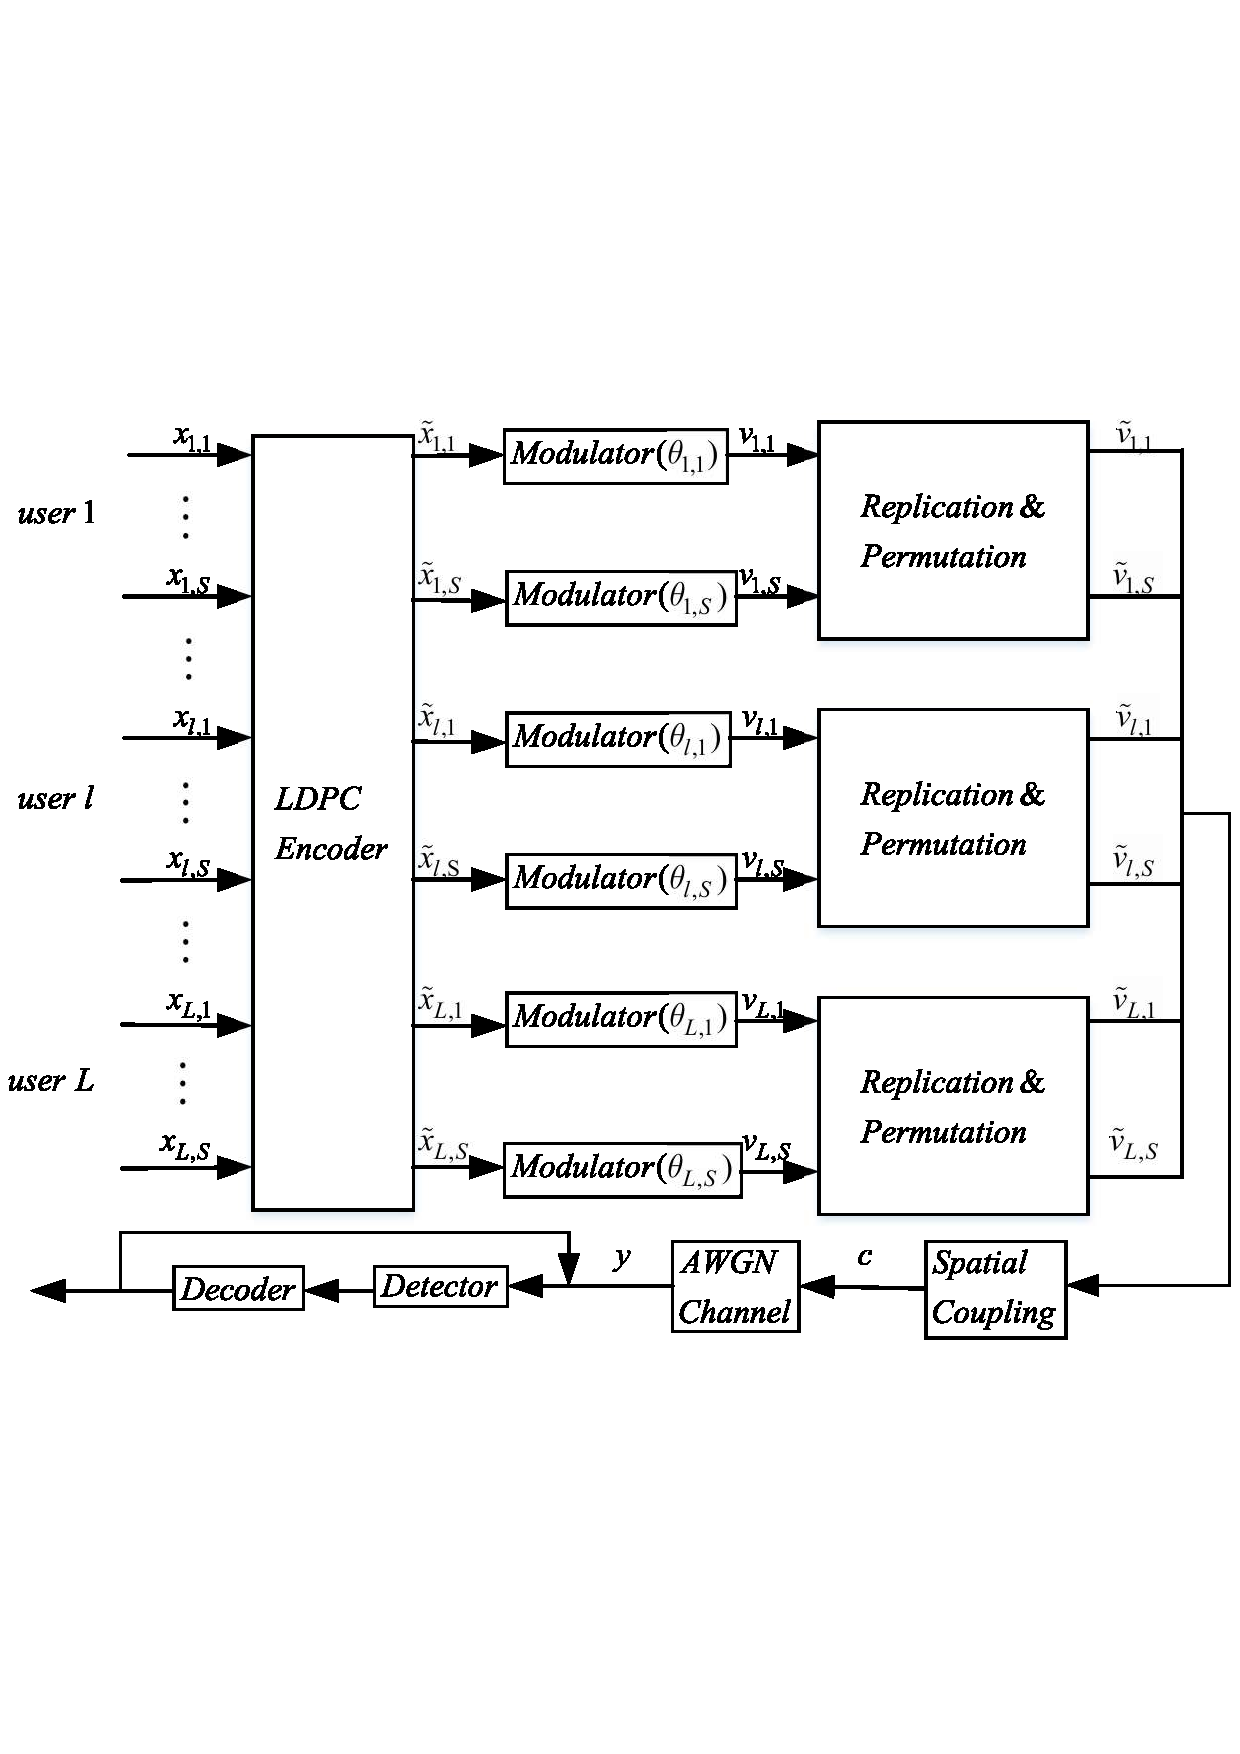
\includegraphics[scale=0.4]{1-4.pdf}}
  \caption{System model of N user each with L streams.}\label{number_inner_iterations}
    \vspace{-1em}
\end{figure}
Without loss of generality, we consider $\left( {2,2,5,3} \right)$-multiuser spatial coupling system. The spatial coupling procedure is represented in Fig. 2, where each row is a data stream of a user and the packages are transmitted one after another. The block ${{\tilde v}^m}_{l,s,p}$ can be denoted as ${{\tilde v}^m}_{l,s,p} = {\pi ^m}_{l,s,p}{v_{l,s,p}}$, where ${\pi ^m}_{l,s,p}$ is the corresponding interleaver. At time $t = 0$, two data streams of the first user start to transmit. The signal transmitted add two data streams of one user each $\tau $ time interval in order until the number of user reaches the limit.
\begin{figure}[h!]
\setlength{\abovecaptionskip}{0.cm}
\setlength{\belowcaptionskip}{-0.cm}
  \centering{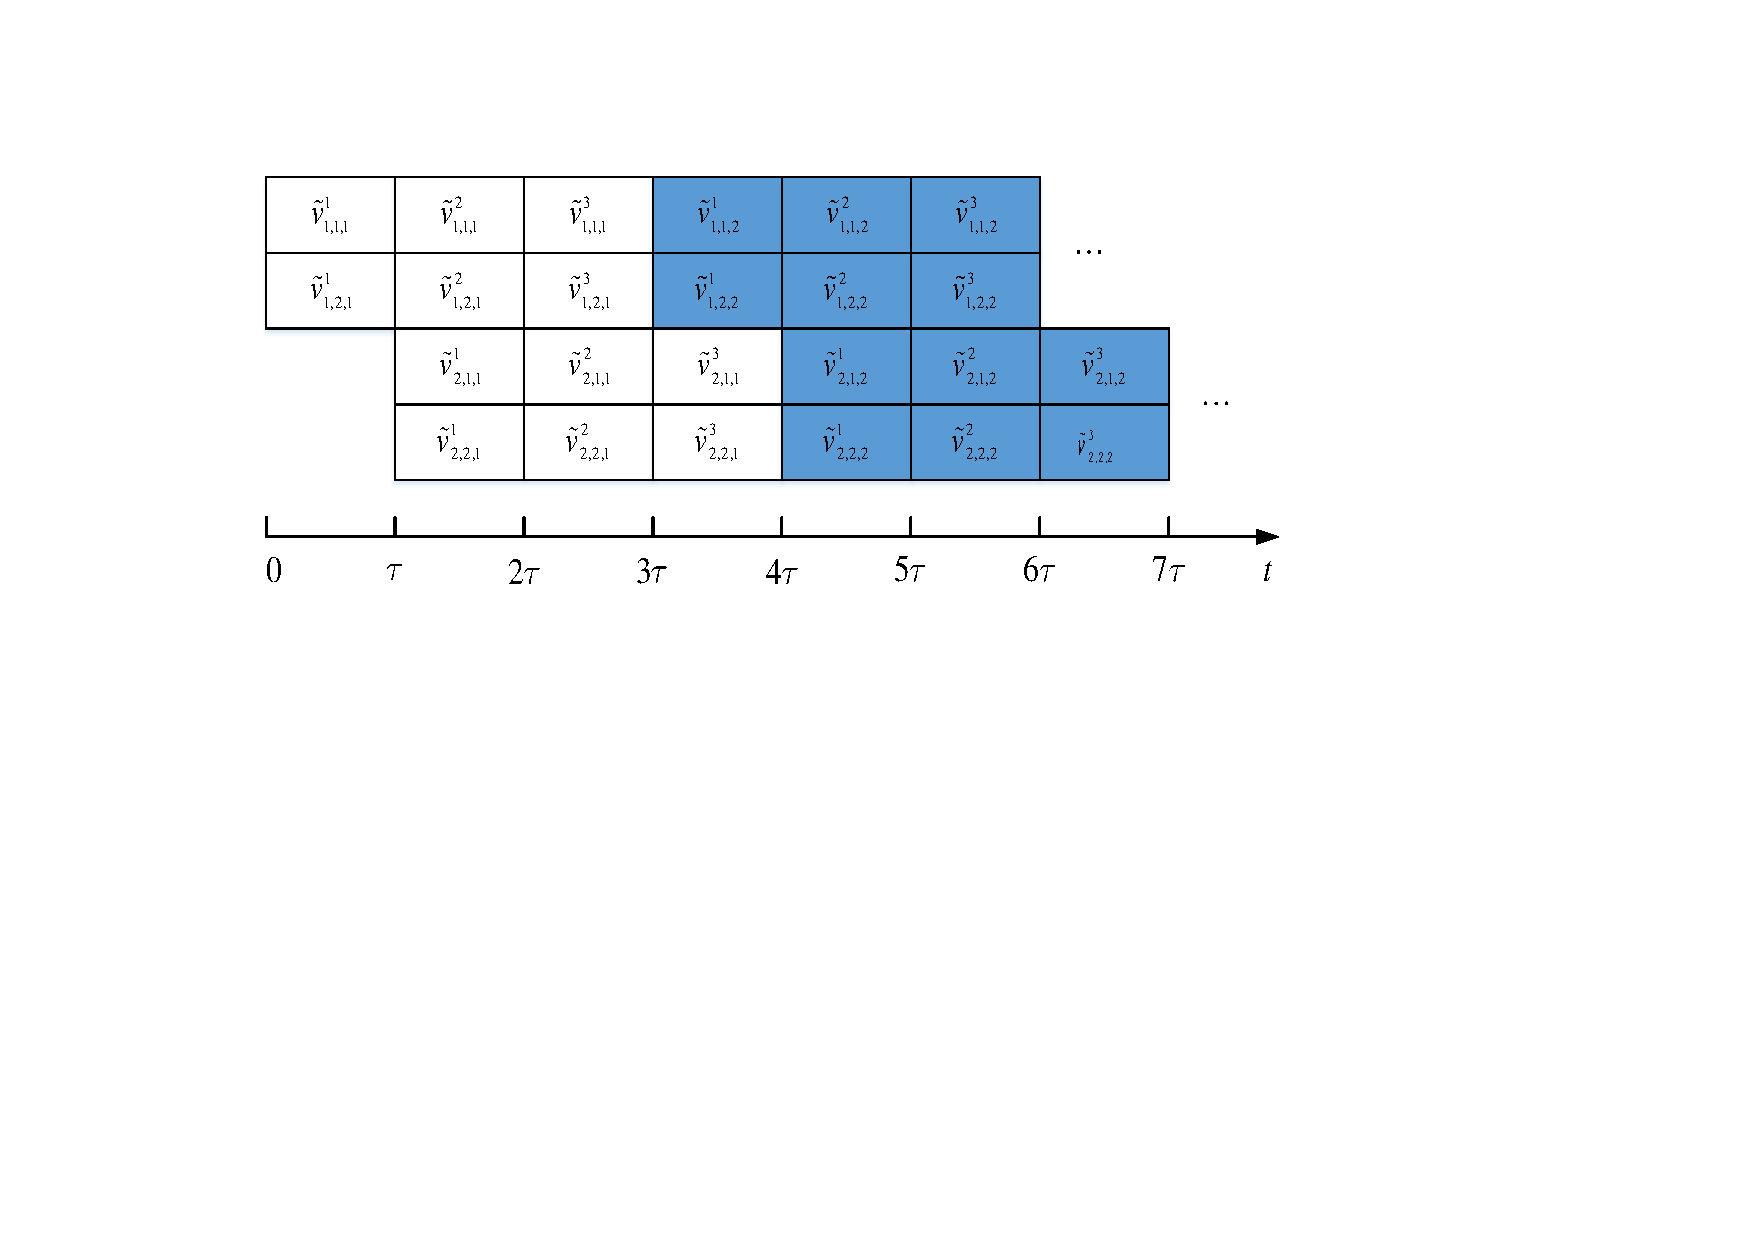
\includegraphics[scale=0.48]{2-1.pdf}}
  \caption{Coupling of modulated data streams with time offset $\tau $ in a $\left( {L,S,P,M} \right)$-multiuser spatial coupling system.}\label{number_inner_iterations}
    \vspace{-1em}
\end{figure}

We use spatial coupling matrix $H$ to achieve above procedure. The construction of $H$ is shown in $(1)$, where ${\pi ^m}_{l,s,p}$ is the permutation matrix of $\pi  \times \pi $ unit matrix. Therefore, the signal $c$ can be described as $c = {H^T}v$,where $v = {\left[ {{v^T}_{1,1,1}, \cdots ,{v^T}_{1,1,P}, \cdots ,{v^T}_{L,S,1}, \cdots ,{v^T}_{L,S,P}} \right]^T}$.
\begin{equation}
\resizebox{.9\hsize}{!}{$H = \left[ {\begin{array}{*{20}{c}}
{{\pi ^1}_{1,1,1}}& \cdots &{{\pi ^M}_{1,1,1}}&{ \cdots  \cdots }&{{\pi ^1}_{1,1,P}}& \cdots &{{\pi ^M}_{1,1,P}}&{}&{}&{}\\
{{\pi ^1}_{1,2,1}}& \cdots &{{\pi ^M}_{1,2,1}}&{ \cdots  \cdots }&{{\pi ^1}_{1,2,P}}& \cdots &{{\pi ^M}_{1,2,P}}&{}&{}&{}\\
 \vdots & \cdots & \vdots &{ \cdots  \cdots }& \vdots & \cdots & \vdots &{}&{}&{}\\
{{\pi ^1}_{1,S,1}}& \cdots &{{\pi ^M}_{1,S,1}}&{ \cdots  \cdots }&{{\pi ^1}_{1,S,P}}& \cdots &{{\pi ^M}_{1,S,P}}&{}&{}&{}\\
{}&{{\pi ^1}_{2,1,1}}& \cdots &{{\pi ^M}_{2,1,1}}&{ \cdots  \cdots }&{{\pi ^1}_{2,1,P}}& \cdots &{{\pi ^M}_{2,1,P}}&{}&{}\\
{}&{{\pi ^1}_{2,2,1}}& \cdots &{{\pi ^M}_{2,2,1}}&{ \cdots  \cdots }&{{\pi ^1}_{2,2,P}}& \cdots &{{\pi ^M}_{2,2,P}}&{}&{}\\
{}& \vdots & \cdots & \vdots &{ \cdots  \cdots }& \vdots & \cdots & \vdots &{}&{}\\
{}&{{\pi ^1}_{2,S,1}}& \cdots &{{\pi ^M}_{2,S,1}}&{ \cdots  \cdots }&{{\pi ^1}_{2,S,P}}& \cdots &{{\pi ^M}_{2,S,P}}&{}&{}\\
{}&{}& \ddots &{}&{}&{}&{}&{}& \ddots &{}\\
{}&{}&{}&{{\pi ^1}_{L,1,1}}& \cdots &{{\pi ^M}_{L,2,1}}&{ \cdots  \cdots }&{{\pi ^1}_{L,1,P}}& \cdots &{{\pi ^M}_{L,1,P}}\\
{}&{}&{}&{{\pi ^1}_{L,2,1}}& \cdots &{{\pi ^M}_{L,2,1}}&{ \cdots  \cdots }&{{\pi ^1}_{L,2,P}}& \cdots &{{\pi ^M}_{L,2,P}}\\
{}&{}&{}& \vdots & \cdots & \vdots &{ \cdots  \cdots }& \vdots & \cdots & \vdots \\
{}&{}&{}&{{\pi ^1}_{L,S,1}}& \cdots &{{\pi ^M}_{L,S,1}}&{ \cdots  \cdots }&{{\pi ^1}_{L,S,P}}& \cdots &{{\pi ^M}_{L,S,P}}
\end{array}} \right]$}
\end{equation}
The total load in the system we proposed is shown in $(2)$, which is actually the ratio between rows and columns of $H$.
\begin{equation}
Load = \frac{{LSPK}}{{\left( {PM + L - 1} \right)K}} = \frac{{LSP}}{{\left( {PM + L - 1} \right)}}
\end{equation}

When the signal is passed through the AWGN channel, channel output can be calculated by $(3)$, where $\lambda $ is the power normalization coefficient, $n$ is gaussian noise, its mean and variance are 0 and ${\sigma ^2}$, respectively.
\begin{equation}
y = \lambda c + n
\end{equation}

At the receiver, iterative detecting and decoding scheme based on message passing algorithm(MPA) is considered. Inner the detector and the decoder, the extrinsic messages are iteratively exchanged along edges between channel nodes and variable nodes. During the iteration between detector and decoder, the output of the detector is transmitted to the decoder, the output of the decoder is used as the input of the detector of next iteration, note that each package of a data stream is encoded and decoded individually. We define the maximum number of iteration as ${I_{\max }}$.

\section{PROPOSED SCHEME}
\subsection{Constellation rotation}
For each data stream, the principle of the constellation rotation we proposed is illestrated in Fig. 4, where the modulated signal is constructed by anticlockwise rotating the signal modulated by BPSK with a certain angle $\theta $. Assuming $x{'_{l,s}}$ denotes the BPSK modulation signal, $x{'_{l,s}} = {\left[ {x{'^T}_{l,s,1},x{'^T}_{l,s,2}, \cdots ,x{'^T}_{l,s,P}} \right]^T}$, then ${v_{l,s}}$ can be described as
\begin{equation}
{v_{l,s}} = {e^{i{\theta _{l,s}}}}x{'_{l,s}}
\end {equation}
\begin{figure}[h!]
\setlength{\abovecaptionskip}{0.cm}
\setlength{\belowcaptionskip}{-0.cm}
  \centering{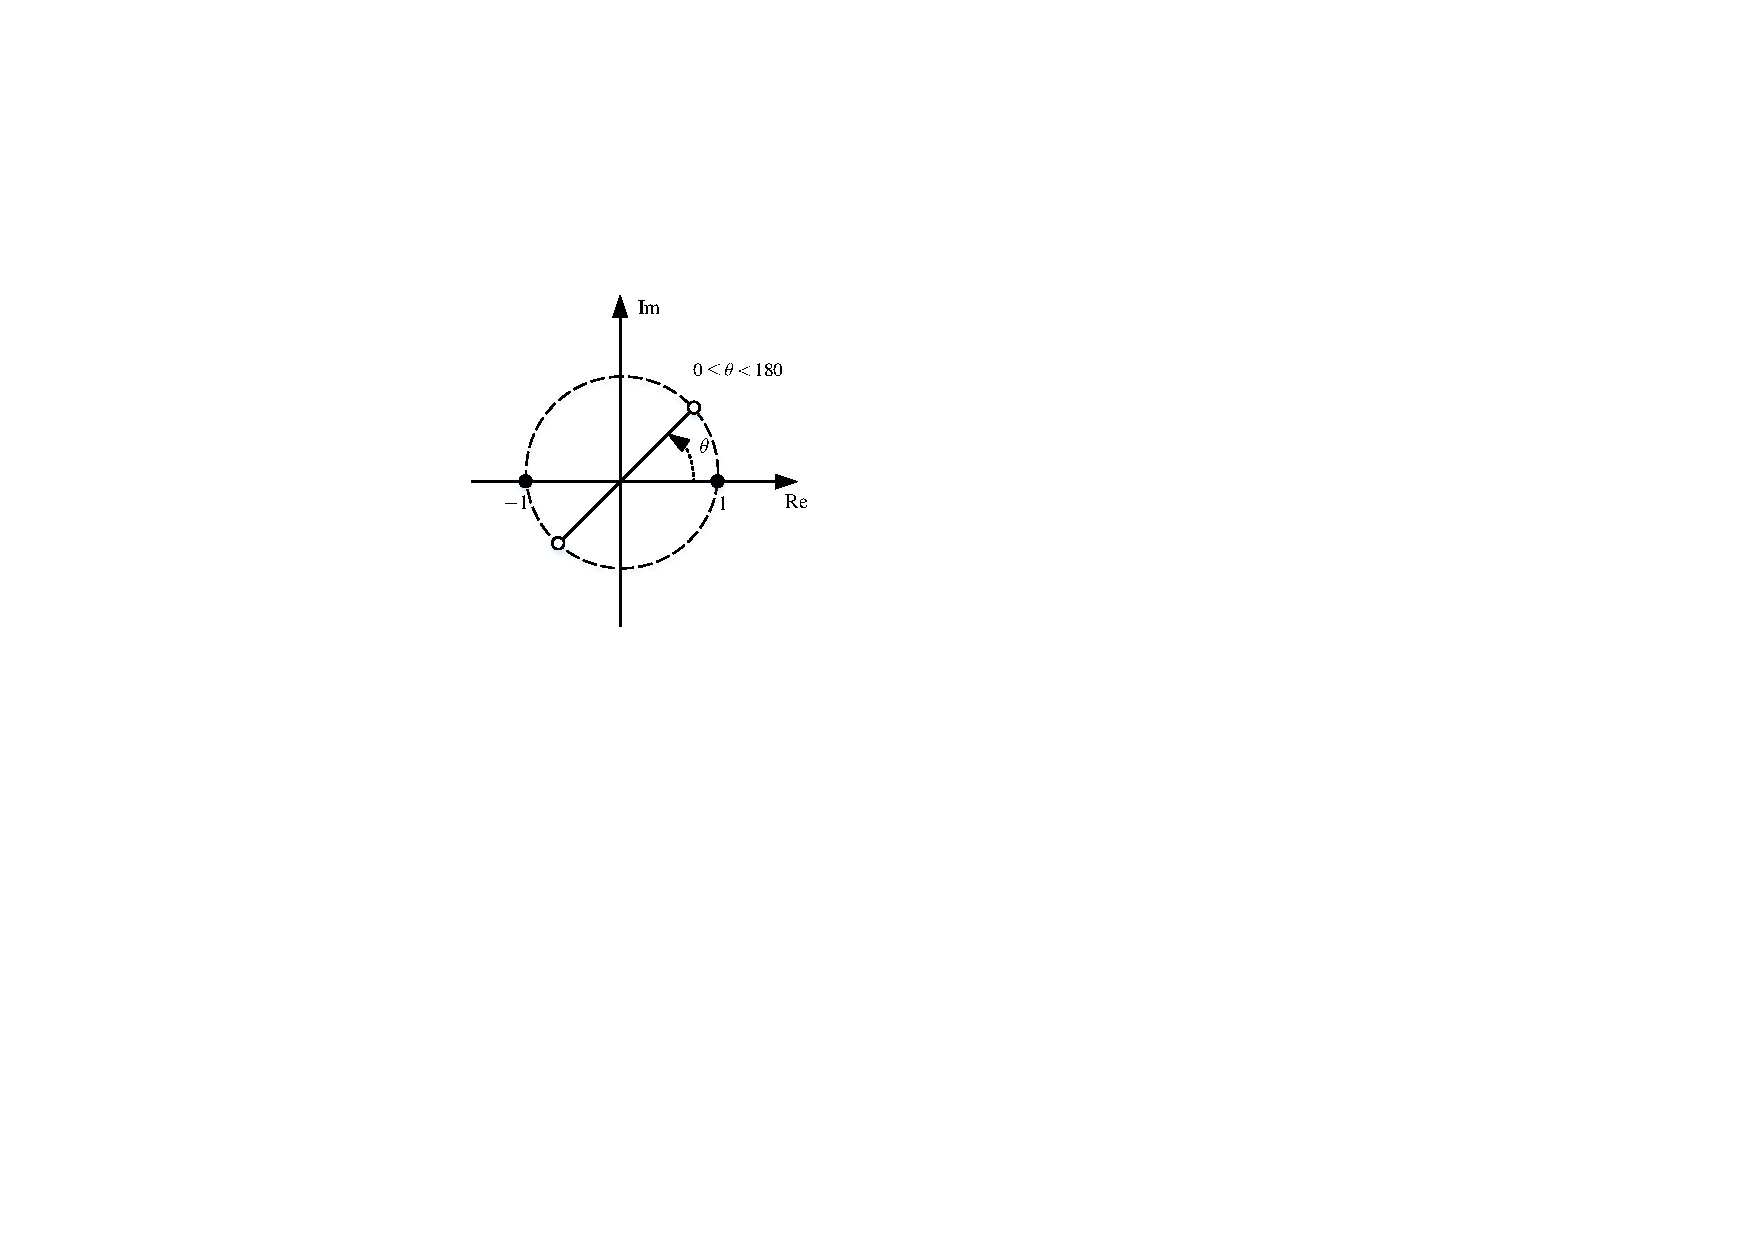
\includegraphics[scale=0.6]{4.pdf}}
  \caption{The constellation rotation of each data stream.}\label{number_inner_iterations}
    \vspace{-1em}
\end{figure}

We illustrate the scheme with the example listed in section \uppercase\expandafter{\romannumeral2} and focus on the constellation of the superimposed signal $c$. In Fig. 5, there are three constellations with different rotation angle set. As can be seen from the figure, we conclude that the constellation of $c$ containing $16$ points when there is no identical angle in the angle set. For the constellation with two or more same rotation angles, some constellation points are overlapping, which lead to the diversity reduction. We call this phenomenon constellation aliasing which make it difficult to distinguish which data streams the superimposed data come from in the detector and lead to performance degradation.
\begin{figure}[h!]
\setlength{\abovecaptionskip}{0.cm}
\setlength{\belowcaptionskip}{-0.cm}
  \centering{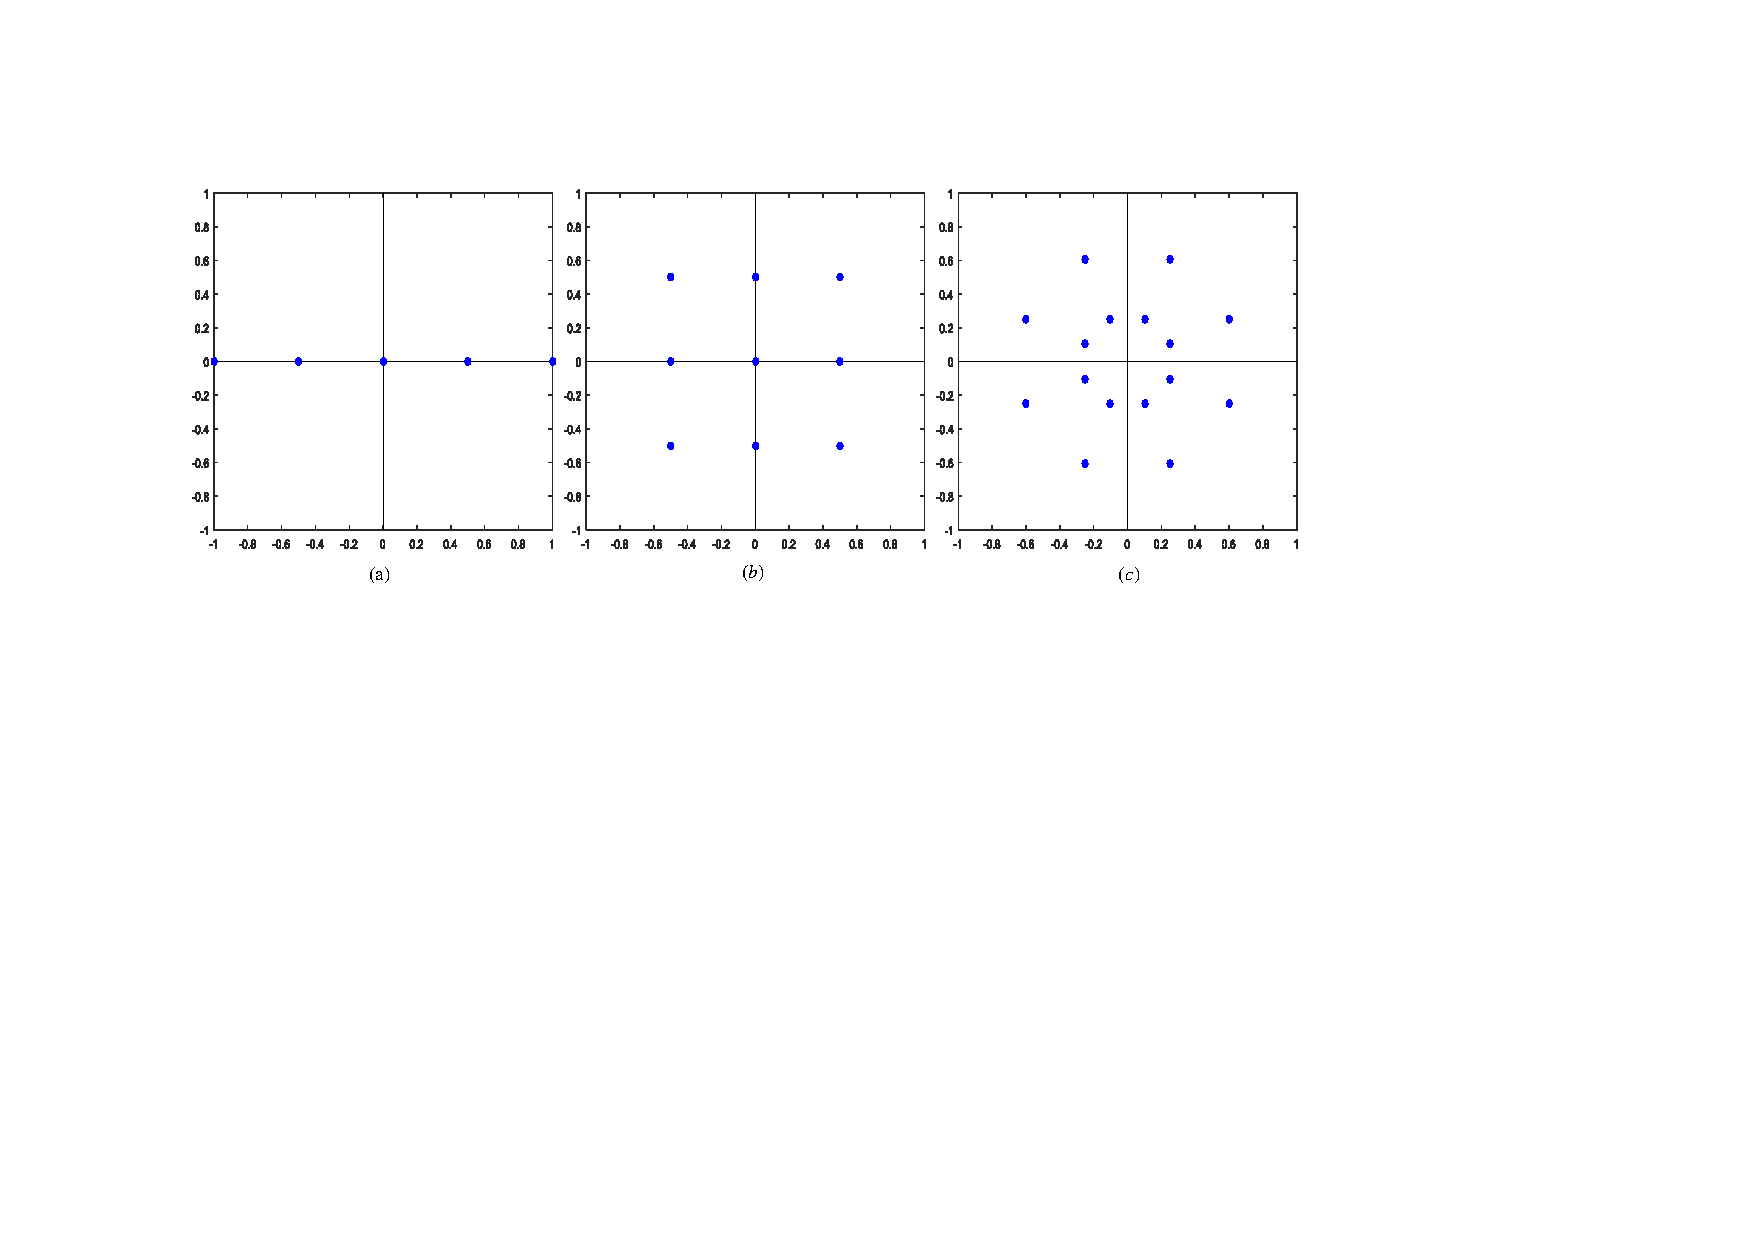
\includegraphics[scale=0.48]{5.pdf}}
  \caption{The constellation of coupled signal $c$. The combinations of rotation angles from left to right are $\left( {0,0,0,0} \right)$, $\left( {0,90,0,90} \right)$, $\left( {0,90,45,135} \right)$, respectively.In case $L = 2$, $S = 2$, $M = 3$.}\label{number_inner_iterations}
    \vspace{-1em}
\end{figure}

When considering constellation, we naturally come up with the minimum Euclidean distance which reflects the mutual interference between constellation points. The shorter the distance is, the greater the interference is. The minimum Euclidean distance decrease when the diversity of the constellation increase. Therefore, it is necessary to make a trade off between constellation aliasing and mutual interference and search for the optimal rotation angle set.
\subsection{Rotation angles optimization}
The optimization of rotation angles is equivalent to find certain angle set with maximum mutual information(MI) between the input $c$ and the output $y$. The maximum MI represents the maximum amount of information about $c$ that can be conveyed through the channel and is also called channel capacity. Assuming the constellation points set of $c$ is denoted by $\left\{ {{c_m}} \right\},\left( {m = 1,2, \cdots ,M} \right)$,${c_m} = {a_m} + i{b_m}$, $y = u + iv$. The channel transition probability is given as
\begin{equation}
\begin{aligned}
p(y|{c_m}) &= \int\int{\frac{1}{{\pi {N_0}}}{e^{ - \;\frac{{{{\left( {u - {a_m}} \right)}^2} + {{\left( {v - {b_m}} \right)}^2}}}{{{N_0}}}}}dudv} \\
&= \int\int\frac{1}{{\pi {N_0}}}{e^{ - \;\frac{{{{\left| {y - {c_m}} \right|}^2}}}{{{N_0}}}}}dudv
\end{aligned}
\end{equation}
Where $N_0$ is the noise power spectral density. In order to facilitate the calculation, we set $N_0$ to 1. The computational formula of MI is derived as
\begin{equation}
\begin{aligned}
I\left( {c;y} \right) = \sum\limits_{m = 1}^M {p\left( {{c_m}} \right)} \int \int p\left( {y|{c_m}} \right)\log \frac{{p\left( {y|{c_m}} \right)}}{{\sum\nolimits_{m = 1}^M {p\left( {{c_m}} \right)p\left( {y|{c_m}} \right)} }}
\end{aligned}
\end{equation}
As $c_m$ occurs with equal probability, we combine $(5)$ with $(6)$, and get the following equation:
\begin{equation}
\begin{aligned}
&I\left( {c;y} \right) = \log M - \\
&\frac{1}{M}\sum\limits_{m = 1}^M {\int\int\frac{1}{{\pi {N_0}}}{e^{ - \;\frac{{{{\left| {y - {c_m}} \right|}^2}}}{{{N_0}}}}}\log \sum\limits_{n = 1}^M {{e^{ - \;\frac{{{{\left| {y - {c_n}} \right|}^2} + {{\left| {y - {c_m}} \right|}^2}}}{{{N_0}}}}}} dudv}
\end{aligned}
\end{equation}

In our scheme, we traverse all sets of rotation angle when the total number of data streams $LS$ is determined and select the optimal rotation angles with the maximum MI.
\subsection{Iterative detecting and decoding}
In this section, we put the process of iteration detecting and decoding scheme in detail. During the detection, the log-likelihood ratios(LLRs) is used as the extrinsic information passed between nodes given in Fig. 5, where circles represent variable nodes corresponding to the data blocks in Fig. 2, channel nodes are coupling data and denoted by squares. The received message of one node along one edge is not allowed to update the message sent on the same edge.
\begin{figure}[h!]
\setlength{\abovecaptionskip}{0.cm}
\setlength{\belowcaptionskip}{-0.cm}
  \centering{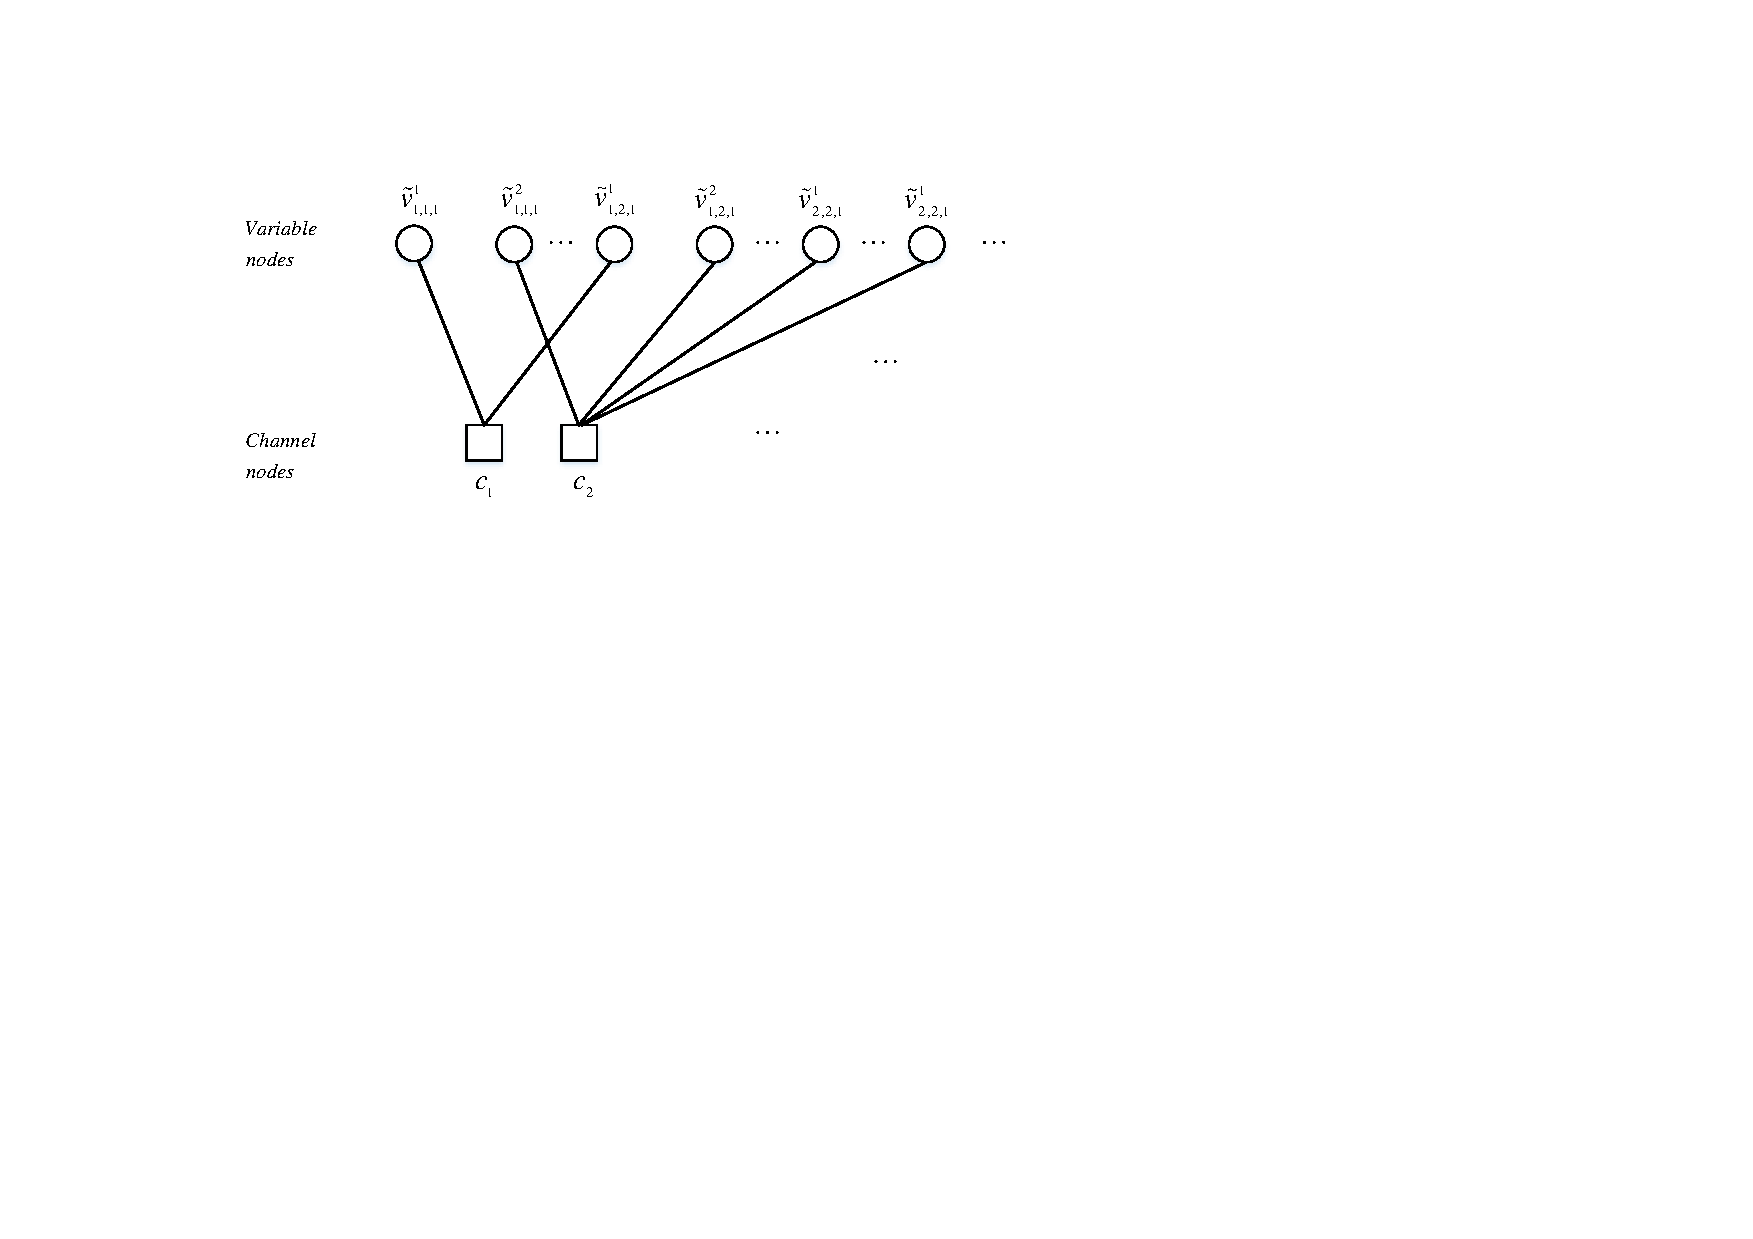
\includegraphics[scale=0.65]{3.pdf}}
  \caption{Factor graph representation of spatial coupling multiple access system corresponding to the Fig .2.}\label{number_inner_iterations}
    \vspace{-1em}
\end{figure}

Let the edge between variable node ${\tilde v_{l,s,p}}$ and channel node ${c_t}$ as observation. Set $\xi (l,s,p)\backslash t$ is the index collection of channel nodes connected with variable node ${\tilde v_{l,s,p}}$ and set $\xi t\backslash (l,s,p)$ is the index collection of variable nodes connected with channel nodes ${c_t}$. Symbol ${l_{{{\tilde v}_{l,s,p}} \to {c_t}}}$ and ${l_{{c_t} \to {{\tilde v}_{l,s,p}}}}$ represents the message sent from ${\tilde v_{l,s,p}}$ and ${c_t}$, respectively. We initialize ${l_{{{\tilde v}_{l,s}} \to {c_t}}}$ as follows
\begin{equation}
{l_{{{\tilde v}_{l,s,p}} \to {c_t}}} = \log \frac{{p(x{'_{l,s,p}} =  + 1)}}{{p(x{'_{l,s,p}} =  - 1)}}
\end{equation}
The message updated during iteration can be write as
\begin{equation}
\begin{aligned}
{l_{{{\tilde v}_{l,s,p}} \to {c_t}}} = \sum\limits_{_{t' \in \xi (l,s,p)\backslash t}} {{l_{{c_{t'}} \to {{\tilde v}_{l,s,p}}}}}
\end{aligned}
\end{equation}
\begin{equation}
\begin{aligned}
{l_{{c_t} \to {{\tilde v}_{l,s,p}}}}\;\;\;{\kern 1pt}  = \;\;\;{\kern 1pt} \log \frac{{p({{\tilde v}_{l,s,p}} =  + {e^{i{\theta _{l,s}}}}|{c_t},{{{\bf{\tilde v}}}^{[t]}}\backslash {{\tilde v}_{l,s,p}})}}{{p({{\tilde v}_{l,s,p}} =  - {e^{i{\theta _{l,s}}}}|{c_t},{{{\bf{\tilde v}}}^{[t]}}\backslash {{\tilde v}_{l,s,p}})}} \\
= \log \frac{{p({c_t}|{{{\bf{\tilde v}}}^{[t]}},{{\tilde v}_{l,s,p}} =  + {e^{i{\theta _{l,s}}}})p({{{\bf{\tilde v}}}^{[t]}}|{{\tilde v}_{l,s,p}} =  + {e^{i{\theta _{l,s}}}})}}{{p({c_t}|{{{\bf{\tilde v}}}^{[t]}},{{\tilde v}_{l,s,p}} =  - {e^{i{\theta _{l,s}}}})p({{{\bf{\tilde v}}}^{[t]}}|{{\tilde v}_{l,s,p}} =  - {e^{i{\theta _{l,s}}}})}}
\end{aligned}
\end{equation}
Where ${{\bf{\tilde v}}^{[t]}}$ denotes the set containing all signals superimposed on the coupled signal ${{c_t}}$. $(10)$ is derived by using Bayes' rule listed below
\begin{equation}
\begin{aligned}
p(x|y) = \frac{{p(y|x)p(x)}}{{p(y)}}\propto p(y|x)p(x)
\end{aligned}
\end{equation}
The conditional probability density function(pdf) of the coupled signal ${{c_t}}$ and the set ${{\textbf{v}^{[t]}}}$ are given separately as
\begin{equation}
p\left( {{c_t}|{{{\bf{\tilde v}}}^{[t]}}} \right) = \frac{1}{{\sqrt {2\pi \sigma } }}\exp \left( { - {\mkern 1mu} \frac{1}{{2{\sigma ^2}}}{{\left\| {{c_t} - {{\bf{h}}^{[t]T}}{{{\bf{\tilde v}}}^{[t]}}} \right\|}^2}} \right)
\end{equation}
\begin{equation}
\begin{aligned}
p\left( {{{{\bf{\tilde v}}}^{[t]}}|{{\tilde v}_{l,s,p}}} \right) = {\prod _{(l',s',p') \in \xi t\backslash (l,s,p)}}p({\tilde v_{l',s',p'}})
\end{aligned}
\end{equation}
where ${\textbf{h}^{[t]}}$ is normalized coefficient vector of ${{\bf{\tilde v}}^{[t]}}$ and a priori probability of ${v_{l',s',p'}}$ is written as
\begin{equation}
p({\tilde v_{l',s',p'}}) = \exp \left( {\frac{{{{\tilde v}_{l',s',p'}}}}{2}{l_{{{\tilde v}_{l',s',p'}} \to {c_t}}}} \right)
\end{equation}
\begin{figure*}[ht]
\begin{equation}
\begin{aligned}
{l_{{c_t} \to {{\tilde v}_{l,s,p}}}} = \mathop {{{\max }^ \star }}\limits_{\begin{array}{*{20}{c}}
{\;\;\;\;\;\;{{{\bf{\tilde v}}}^{[t]}}\;\;\;\;\;\;}\\
{{{\tilde v}_{l,s,p}} =  + {e^{i{\theta _{l,s}}}}}
\end{array}} \left( {{\sum _{(l',s',p') \in \xi t\backslash (l,s,p)}}\frac{{{{\tilde v}_{l,s,p}}}}{2}{l_{{{\tilde v}_{l,s,p}} \to {c_t}}} - \frac{1}{{2{\sigma ^2}}}{{\left\| {{c_t} - {{\bf{h}}^{[t]T}}{{{\bf{\tilde v}}}^{[t]}}} \right\|}^2}} \right) \\- \mathop {{{\max }^ \star }}\limits_{\begin{array}{*{20}{c}}
{\;\;\;\;\;\;{{{\bf{\tilde v}}}^{[t]}}\;\;\;\;\;\;}\\
{{{\tilde v}_{l,s,p}} =  - {e^{i{\theta _{l,s}}}}}
\end{array}} \left( {{\sum _{(l',s',p') \in \xi t\backslash (l,s,p)}}\frac{{{{\tilde v}_{l,s,p}}}}{2}{l_{{{\tilde v}_{l,s,p}} \to {c_t}}} - \frac{1}{{2{\sigma ^2}}}{{\left\| {{c_t} - {{\bf{h}}^{[t]T}}{{{\bf{\tilde v}}}^{[t]}}} \right\|}^2}} \right)
\end{aligned}
\end{equation}
\end{figure*}
Substituting $(12)$, $(13)$ and $(14)$ into $(10)$, we get $(15)$ shown on the top of this page, where ${\mathop {\max }\nolimits^* }$ operation\cite{12} is defined as follows:
\begin{equation}
\begin{aligned}
\mathop {\max }\nolimits^* (a,b) &= \log (\exp (a) + \exp (b)) \\&= \max(a,b) + \log(1 + \exp ( - \left| {a - b} \right|))
\end{aligned}
\end{equation}
We define the iterative process from the detector to the decoder as a whole iteration. The message exchanged between detector and decoder can be described as
\begin{equation}
\begin{aligned}
l_{out,{{\tilde v}_{l,s,p}}}^{DEC[i]} = l_{{{\tilde v}_{l,s,p}}}^{{I_{DEC}}} - l_{out,{{\tilde v}_{l,s,p}}}^{DET[i]}
\end{aligned}
\end{equation}
where the symbol on the left of the equal sign represents the output of the decoder in $i$th iteration, $i \in \left[ {1, \cdots {I_{\max }}} \right]$. On the right side, the subtrahend is the LLRs of the decoder after ${{I_{DEC}}}$ inner iterations and is used for soft decision, the minuend denotes the output of the detector in $i$th iteration, initializes to $0$ when $i=1$ and is update as
\begin{equation}
\begin{aligned}
l_{out,{{\tilde v}_{l,s,p}}}^{DET[i]} = l_{{{\tilde v}_{l,s,p}}}^{{I_{DET}}} - l_{out,{{\tilde v}_{l,s,p}}}^{DEC[i - 1]}
\end{aligned}
\end{equation}
where $l_{{{\tilde v}_{l,s,p}}}^{{I_{DET}}}$ is the total LLRs received from neighbors of ${{{\tilde v}_{l,s,p}}}$ after ${{I_{DET}}}$ iterations. The symbol $l_{out,{{\tilde v}_{l,s,p}}}^{DEC[i - 1]}$ is the ${i - 1}$th iterative output of the detector.

\section{SIMULATION RESULTS}
In this section, we analyze the system performance using EXIT charts and BER curves. We have verified that our constellation rotation is also applicable to any $\left( {3,2,5,2} \right)$-multiuser spatial coupling structure. To facilitate the analysis, we take $\left( {2,2,5,2} \right)$-multiuser spatial coupling system as observation, the encoding scheme considered is $(3,6)$-regular LDPC code with length $N=1800$ and rate ${1 \mathord{\left/
 {\vphantom {1 2}} \right.
 \kern-\nulldelimiterspace} 2}$ and the maximum inner iteration in the detector and the decoder are $2$ and $10$. The optimal rotation angle set we seek out is $(0,90,45,135)$.
\subsection{EXIT chart}
EXIT chart is a useful tool to track the mutual information at each iteration between soft-in soft-out(SISO) constituents, and it provides an excellent prediction on the behavior of the iteration. We use EXIT charts to evaluate the performance of the detector(or the decoder) by observing whether it is conductive to increase the output mutual information ${I_E}$ when the input extrinsic information ${I_A}$ is given. We produce the EXIT curve with several input mutual information and the corresponding output of detector(or decoder).

There are two EXIT curves of detector with different rotation angle set over AWGN channel at ${{{E_b}} \mathord{\left/
 {\vphantom {{{E_b}} {{N_0}}}} \right.
 \kern-\nulldelimiterspace} {{N_0}}} = 4dB$ shown in Fig. 6 and ${{{E_b}} \mathord{\left/
 {\vphantom {{{E_b}} {{N_0}}}} \right.
 \kern-\nulldelimiterspace} {{N_0}}} = 8dB$ shown in Fig. 7, respectively.
\begin{figure}[h!]
\setlength{\abovecaptionskip}{0.cm}
\setlength{\belowcaptionskip}{-0.cm}
  \centering{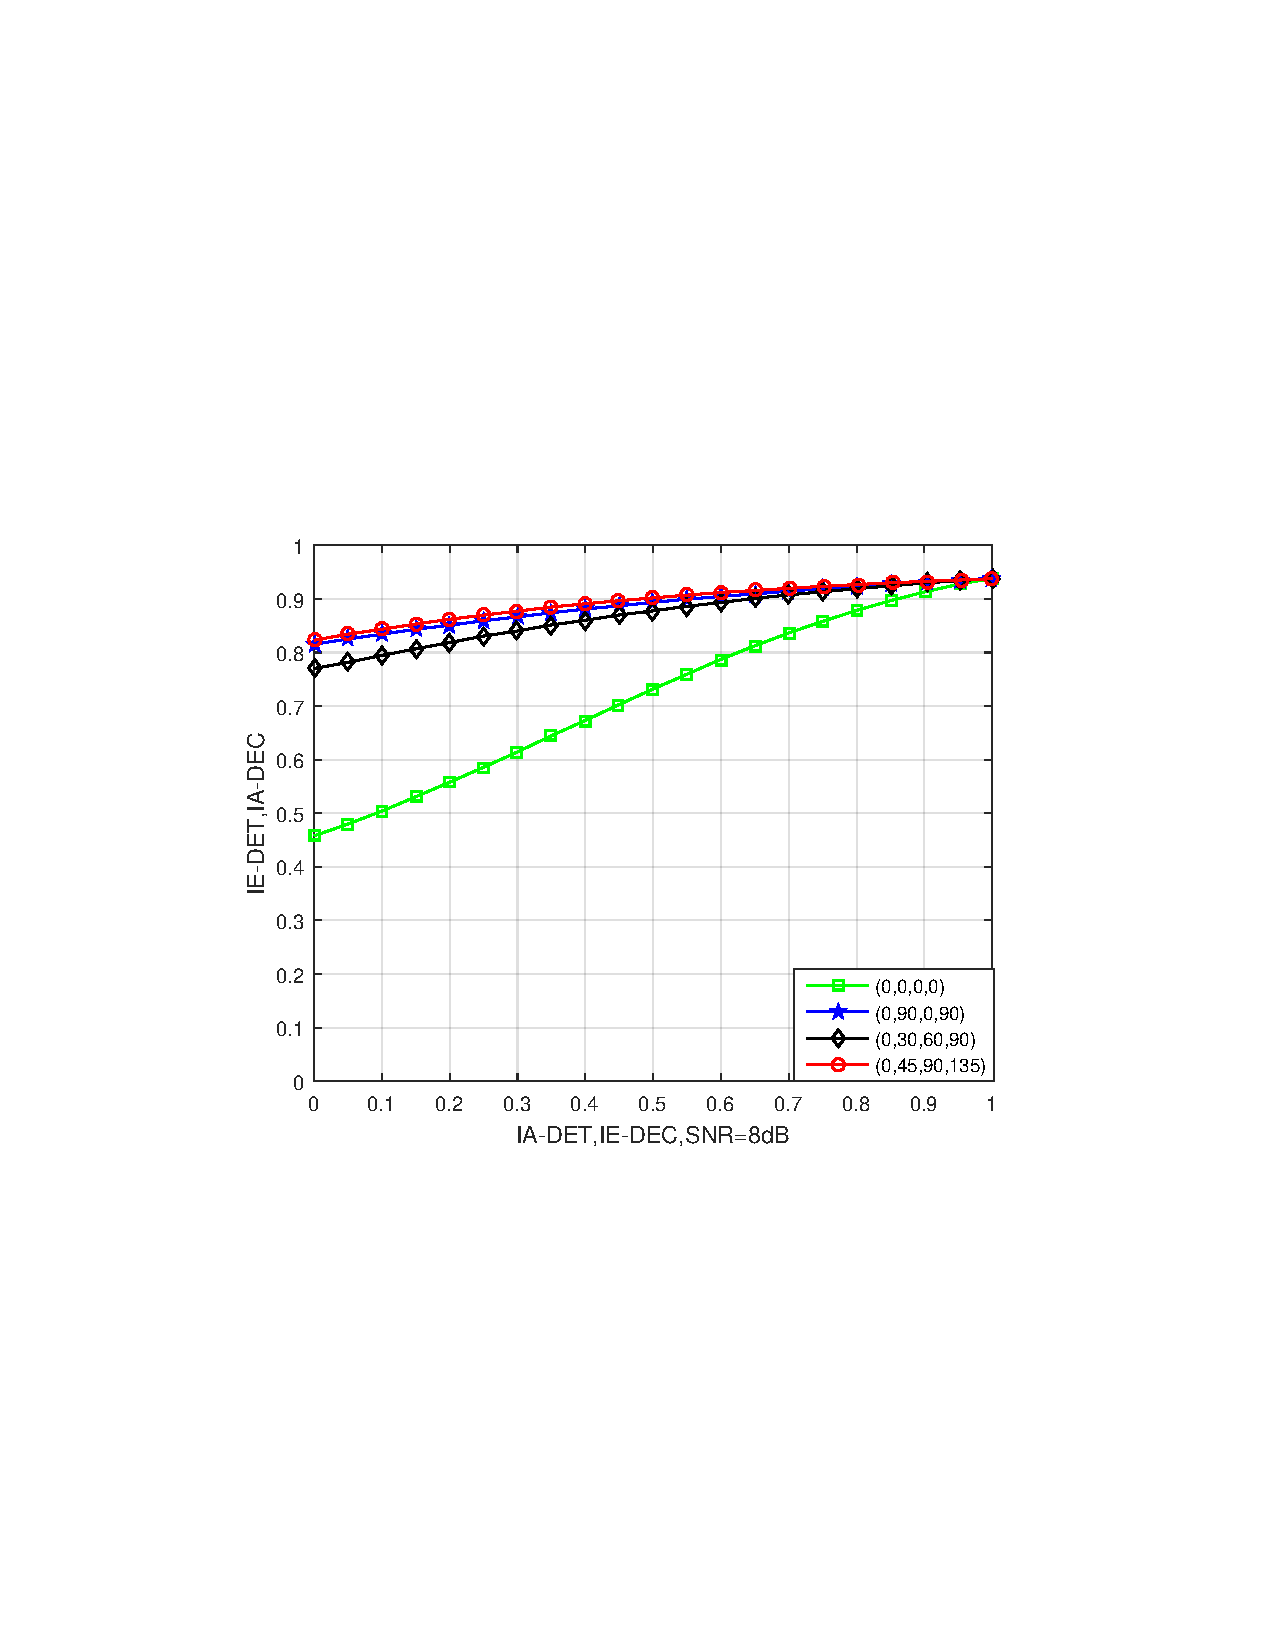
\includegraphics[scale=0.6]{6-1.pdf}}
  \caption{The EXIT chart of the detector with $2$ inner iterations for different rotation angle group in $\left( {2,2,5,2} \right)$-multiuser spatial coupling system with ${E_b}/{N_0} = 3dB$.}\label{number_inner_iterations}
    \vspace{-1em}
\end{figure}
\begin{figure}[h!]
\setlength{\abovecaptionskip}{0.cm}
\setlength{\belowcaptionskip}{-0.cm}
  \centering{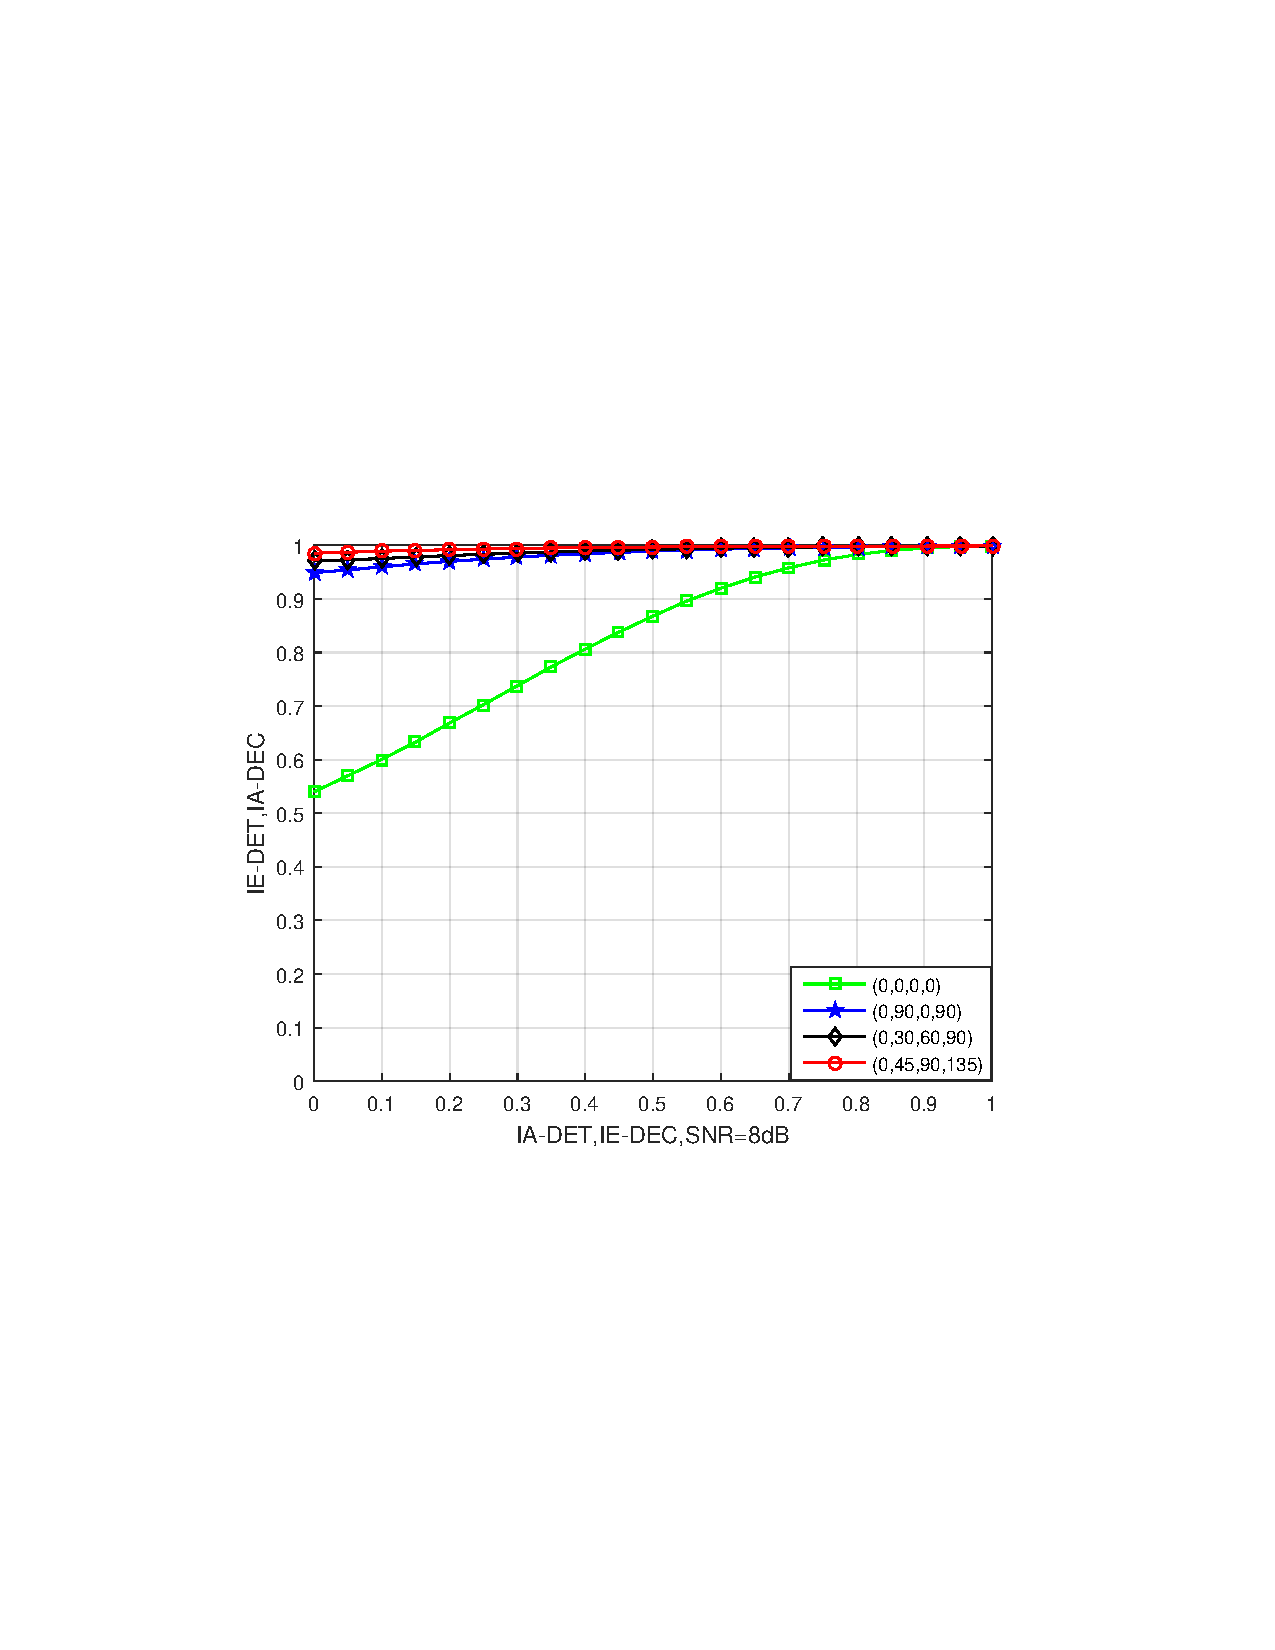
\includegraphics[scale=0.6]{6-22.pdf}}
  \caption{The EXIT chart of the detector with $2$ inner iterations for different rotation angle group in $\left( {2,2,5,2} \right)$-multiuser spatial coupling system with ${E_b}/{N_0} = 8dB$.}\label{number_inner_iterations}
    \vspace{-1em}
\end{figure}
According to the figures, we reach a conclusion that constellation rotation does contribute to increase the output mutual information of the detector. The system performance is influenced by the rotation angle set, for $(0,90,0,90)$, namely, two data streams of a user are perpendicular to each other, which means that there exists no interference between certain user's different data streams, but the interference between the two users can not be eliminated and results in the constellation aliasing. For the set randomly selected, such as $(0,30,60,90)$, each data stream is rotated with different angles which expands diversity, but interference exists between all data streams. It can be seen that when the SNR is low at $4dB$, the performance of detector is better for $(0,90,0,90)$, that is to say interference plays a dominant role in the factors affecting the performance rather than diversity. On the contrary, when the SNR is high at $8dB$, the performance of detector is better for $(0,30,60,90)$, which means diversity is the main influencing factor. For the optimal angle set selected by using the method we proposed, the output mutual information of the detector is both larger than the others at $4dB$ and $8dB$.
% conference papers do not normally have an appendix
\subsection{BER curve}
BER curve can visually describe the performance of the system. We illustrate the average BER curve of the system in Fig. 8, where dotted line and solid line represent the system with ${I_{\max }} = 12$ and ${I_{\max }} = 20$ iterations between detector and decoder respectively. When the number of iteration is fixed, it can be observed that the system with constellation rotation improves its performance indeed and rotation angle set $\left( {0,90,45,135} \right)$ achieve the optimal BER performance, which is consistent with the analysis of EXIT charts above. Compared with the system without constellation rotation, there exists about $2.3dB$ performance improvement.
The system with fixed rotation angle set achieves better performance as ${I_{\max }}$ increases. And the performance of the system with constellation rotation converges faster, which is beneficial to reduce the implementation complexity and latency of the system.
\begin{figure}[h!]
\setlength{\abovecaptionskip}{0.cm}
\setlength{\belowcaptionskip}{-0.cm}
  \centering{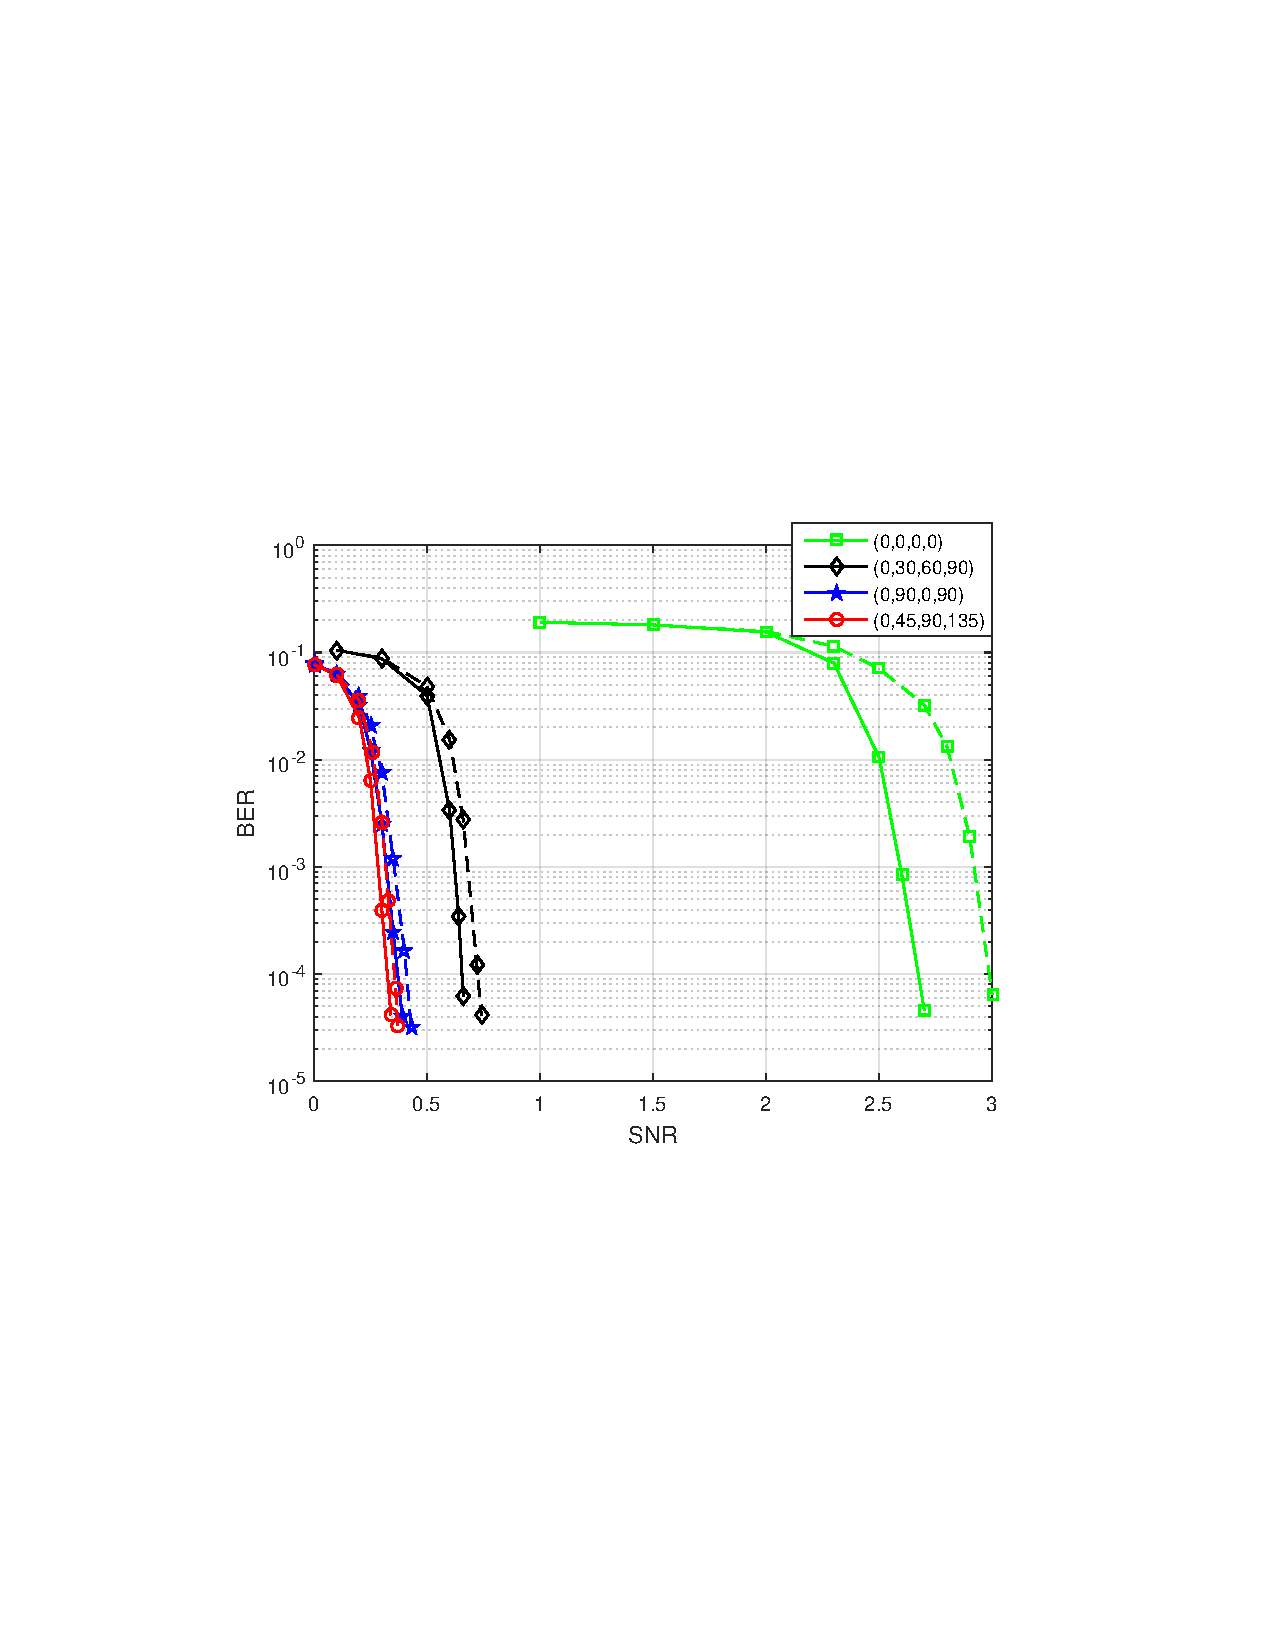
\includegraphics[scale=0.68]{7-1.pdf}}
  \caption{The average BER curve of $\left( {2,2,5,2} \right)$-multiuser spatial coupling system with different rotation angle groups and different iterations between detector and decoder.}\label{number_inner_iterations}
    \vspace{-1em}
\end{figure}
\section*{CONCLUSION}
In this paper, we have applied constellation rotation in spatial coupling multiple access system with LDPC codes and iterative detecting and decoding scheme, and sought out the optimal rotation angle set with the help of mutual information. The EXIT charts and BER curve simulation results verify that the constellation rotation benefits to improve the performance of the system and reduce the implementation complexity and latency, the system with the optimal rotation angle set performs significantly better than the others.
% use section* for acknowledgment
%\section*{Acknowledgment}


%The authors would like to thank...





% trigger a \newpage just before the given reference
% number - used to balance the columns on the last page
% adjust value as needed - may need to be readjusted if
% the document is modified later
%\IEEEtriggeratref{8}
% The "triggered" command can be changed if desired:
%\IEEEtriggercmd{\enlargethispage{-5in}}

% references section

% can use a bibliography generated by BibTeX as a .bbl file
% BibTeX documentation can be easily obtained at:
% http://www.ctan.org/tex-archive/biblio/bibtex/contrib/doc/
% The IEEEtran BibTeX style support page is at:
% http://www.michaelshell.org/tex/ieeetran/bibtex/
%\bibliographystyle{IEEEtran}
% argument is your BibTeX string definitions and bibliography database(s)
%\bibliography{IEEEabrv,../bib/paper}
%
% <OR> manually copy in the resultant .bbl file
% set second argument of \begin to the number of references
% (used to reserve space for the reference number labels box)
\begin{thebibliography}{100}

\bibitem{1}
L. Dai, B. Wang, Y. Yuan, S. Han, C. I and Z. Wang, "Non-orthogonal multiple access for 5G: solutions, challenges, opportunities, and future research trends," in IEEE Communications Magazine, vol.53, no. 9, pp. 74-81, Sep. 2015.
\bibitem{2}
C. Yan, A. Harada, A. Benjebbour, Y. Lan, A. Li and H. Jiang, "Receiver
design for downlink non-orthogonal multiple access (NOMA)," IEEE VTC Spring 2015, May 2015.
\bibitem{3}
M. -R. Hojeij, J. Farah, C. A. Nour and C. Douillard, "Resource allocation in downlink non-orthogonal multiple access (NOMA) for future radio access," IEEE VTC Spring 2015, May 2015.
\bibitem{4}
D. Truhachev, M. Lentmaier, and K. S. Zigangirov, "Mathematical analysis of iterative decoding of ldpc convolutional codes," in Proccedings of the 2001 IEEE International Symposium on Information Theory, Washington, USA, June 2001.

\bibitem{5}
M. Lentmaier, A. Sridharan, D. J. Costello, and K. S. Zigangirov, "Iterative decoding threshold analysis for LDPC convolutional codes," IEEE Trans. Inform. Theory, vol. 56, pp. 5274�C5289, Oct. 2010.

\bibitem{6}
D. Truhachev, "Universal multiple access via spatially coupling data transmission," in Proc. IEEE Int. Symp. Inf. Theory (ISIT), Jul. 2013, pp. 1884�C1888.
\bibitem{7}
K. Takeuchi, T. Tanaka, and T. Kawabata, "Performance Improvement of Iterative Multiuser Detection for Large Sparsely Spread CDMA Systems by Spatial Coupling," IEEE Trans. Inf. Theory, vol. 61, no. 4, pp. 1768-1794, Apr. 2015.
\bibitem{8}
C. Schlegel and D. Truhachev, "Multiple access demodulation in the lifted signal graph with spatial coupling," IEEE Trans. Inf. Theory, vol. 59, no. 4, pp. 2459�C2470, Apr. 2013.

\bibitem{9}
Soumya Sunder Dash, Frederic Pythoud, Benedikt Baeuerle, Arne Josten, Pascal Leuchtmann, David Hillerkuss and Juerg Leuthold, "Approaching the Shannon Limit Through Constellation Modulation," Optical Fiber Communications Conference and Exhibition (OFC), Aug. 2016.

%8Approaching the Shannon Limit Through Constellation Modulation
%9Multi-dimensional SCMA Codebook Design Based on Constellation Rotation and Interleaving
\bibitem{10}
D. Cai, P. Fan, X. Lei, Y. Liu, and D. Chen, "Multi-dimensional SCMA codebook  design  based  on  constellation  rotation  and  interleaving," in Proc. IEEE 83rd Veh. Technol. Conf. (VTC Spring), May 2016, pp. 1�C5.
\bibitem{11}
R. G. Gallager, "Low-density parity-check codes," IRE Trans. Inform. Theory, vol. IT-8, pp. 21�C28, Jan. 1962.
\bibitem{12}
R. Hoshyar, F.Wathan, and R. Tafazolli,"Novel low-density signature for synchronous CDMA systems over AWGN channel," IEEE Trans. Signal Process., vol.
56, no. 4, pp. 1616C1626, Apr. 2008.
\end{thebibliography}




% that's all folks
\end{document}


